\documentclass[hidelinks,12pt]{article}
\pdfoutput=1
\usepackage{epsfig,amsfonts,amssymb}

\usepackage{comment}
\input epsf.sty
\topmargin -.1cm
\textheight 21cm
\oddsidemargin 0.15cm 
\textwidth 14cm
\usepackage{cite}
\usepackage{epsfig,amssymb,euscript,xspace,xcolor}
\usepackage{amsmath,mathtools,empheq,amsthm,hyperref,graphicx,paralist}
\usepackage{mathrsfs,float}  
\usepackage{pgf,tikz,pgfplots}
\usetikzlibrary{arrows}
\usepackage[T1]{fontenc} 
\usepackage{tikz,caption,subcaption,marvosym} 
\usetikzlibrary{decorations.markings,arrows,snakes}
\usepackage[belowskip=-15pt,aboveskip=0pt]{caption}
\usepackage[skip=10pt]{caption} % example skip set to 2pt
\usepackage{comment}


\usepackage{enumitem} 


\usepackage[utf8]{inputenc}

\usepackage[titles]{tocloft}
\renewcommand{\cftdot}{} %Don't want dots in TOC


\definecolor{lightblue}{rgb}{.1,.4,.5}
\definecolor{brown1}{rgb}{.64,.43,.138}

\usepackage{hyperref,cite}
\hypersetup{linktocpage, colorlinks=true,linkcolor= blue,citecolor=blue,urlcolor=lightblue}

\newcommand{\hab}{}

\newcommand{\pii}{\pi}

\newcommand{\vq}{\xi}

\newcommand{\tree}{}

\newcommand{\epk}{\epsilon^{\mu\nu}p_{\nu}k^{\rho}k^{\sigma}}
\newcommand{\epkl}{(p. k)\epsilon^{\mu\rho}k^{\sigma}}
\newcommand{\epkll}{\epsilon^{\mu\rho}p_{\rho}k^{\nu}k^{\sigma}}
\newcommand{\epklll}{\epsilon^{\mu\nu}p_{\rho}k^{\rho}k^{\sigma}}

\textwidth 16.9cm
\oddsidemargin -.25cm

\def\ZZZ{{\hbox{ Z\kern-1.6mm Z}}}
\def\RRR{{\hbox{ R\kern-2.4mm R}}}
\def\CCC{{\hbox{ C\kern-2.0mm C}}}
\def\zzz{{\hbox{z\kern-1mm z}}}
\def\eee{e}

\newcommand{\ten}{{(10)}}
\newcommand{\bet}{{( b )}}

\newcommand{\qq}{k}
\newcommand{\pp}{l}
\newcommand{\nn}{\nonumber \\ }

\newcommand{\vt}{\vartheta}

\newcommand{\vtau} {\vec \tau}
\newcommand{\vj} {\vec J}
\newcommand{\vxi} {\vec \xi}
\newcommand{\vu} {\vec u}
\newcommand{\htau} {\vec \eta}
\newcommand{\vc}{\vec\chi}
\newcommand{\vpsi} {\vec \psi}

\newcommand{\qeq}{{\hbox{=\kern-2.3mm ? \kern.5mm }}}
\renewcommand{\qeq}{=}
\usepackage{tikz}
\newcommand*\circled[1]{\tikz[baseline=(char.base)]{\node[shape=circle,draw,inner sep=2pt] (char){#1};}}

\newcommand{\rrho}{r}
\newcommand{\bA}{{\bf A}}
\newcommand{\tx}{\wt x}
\newcommand{\bG}{{\bf G}}
\newcommand{\bF}{{\bar F}}
\newcommand{\bbb}{{\bar b}}
\newcommand{\gam}{\tau}
\newcommand{\eps}{\epsilon}
\newcommand{\vareps}{\varepsilon}
\newcommand{\ra}{\rangle}
\newcommand{\la}{\langle}
\newcommand{\T}{\chi_{T}(k)}
\newcommand{\Tm}{\chi_{T}(k')}
\newcommand{\Cn}{{\cal C}_n}
\newcommand{\vp}{\varphi}
\newcommand{\ve}{\varepsilon}
\newcommand{\tl}{\lambda}
\newcommand{\dt}{(\vec \nabla T)^2}
\newcommand{\hp}{{\wh\Phi}}
\newcommand{\hq}{{\wh Q_B}}
\newcommand{\he}{{\wh\eta_0}}
\newcommand{\ha}{{\wh{A}}}
\newcommand{\lllb}{\Bigl\langle\Bigl\langle}
\newcommand{\rrrb}{\Bigr\rangle\Bigr\rangle}
\newcommand{\tf}{\wt f}
\newcommand{\sss}{{\cal L}_{av}}
\newcommand{\bx}{\bar x}
\newcommand{\bw}{\bar w}
\newcommand{\ws}{{\wt\sigma}}
\newcommand{\wrh}{{\wt\rho}}
\newcommand{\wv}{{\wt v}}

\newcommand{\bJ}{{\bf J}}




\newcommand{\vv} {\bar v}
\newcommand{\uu} {\bar u}

\newcommand{\K}{{\rm K_1}}
\newcommand{\Kt}{{\rm \widetilde K_1}}

\newcommand{\B}{b'}
\newcommand{\C}{c\,'}
\newcommand{\bB}{\bar b'}
\newcommand{\Bu}{B_{\vec u}}
\newcommand{\VV}{{\cal V}}
\newcommand{\BB}{{\cal B}}
\newcommand{\DD}{{\cal D}}
\newcommand{\BBB}{{\cal B}}
\newcommand{\II}{{\cal I}}
\newcommand{\AAA}{{\cal A}}
\newcommand{\GG}{{\cal G}}
\newcommand{\KK}{{\cal K}}
\newcommand{\fff}{{\bf f}}
\newcommand{\ccc}{{\bf c}}
\newcommand{\FF}{{\cal F}}
\newcommand{\JJ}{{\cal J}}
\newcommand{\HH}{{\cal H}}
\newcommand{\MM}{{\cal M}}
\newcommand{\CC}{{\cal C}}
\newcommand{\bC}{{\bf C}}
\newcommand{\OO}{{\cal O}}
\newcommand{\QQ}{{\cal Q}}
\newcommand{\PP}{{\cal P}}
\newcommand{\EE}{{\cal E}}
\newcommand{\LL}{{\cal L}}

\newcommand{\XX}{{\cal X}}

\newcommand{\rrr}{\rangle\rangle}
\newcommand{\half}{{1\over 2}}
\newcommand{\wt}{\widetilde}
\newcommand{\wh}{\widehat}
\newcommand{\wc}{\wt}
\newcommand{\wb}{\bar}
%\newcommand{\bd}{\bar{\rm D}}
\newcommand{\RR}{{\cal R}}
\newcommand{\NN}{{\cal N}}
\newcommand{\TT}{{\cal T}}
\newcommand{\bg}{\bar g}
\newcommand{\ba}{\bar a}
\newcommand{\bc}{\bar c}
\newcommand{\bd}{\bar d}
\newcommand{\bb}{\bar b}
\newcommand{\bT}{\bar \Theta}
\newcommand{\SSS}{{\cal S}}
\newcommand{\tlx}{\left(\tilde \lambda ; X^0(0) \right)}
\newcommand{\al}{\alpha}

\newcommand{\tk}{\tilde \kappa}

%\newcommand{\gcd}{{\rm gcd}}
\newcommand{\ppp}{\prime\prime}

\newcommand{\omk}{\omega_n(\vec k)}
\newcommand{\onk}{\omega^{(N)}_{\vec k_\perp}}
\newcommand{\tI}{\wt\II}
\newcommand{\hI}{\wh\II}
\newcommand{\nI}{\II}

\newcommand{\cp}{\check\Phi}
\newcommand{\cps}{\Psi}
\newcommand{\crh}{\check\rho}
\newcommand{\cs}{\check\sigma}
\newcommand{\cv}{\check v}
\newcommand{\com}{\check\Omega}

\newcommand{\be}{\begin{equation}}
\newcommand{\ee}{\end{equation}}
\newcommand{\ben}{\begin{eqnarray}\displaystyle}
\newcommand{\een}{\end{eqnarray}}

\newcommand{\refb}[1]{(\ref{#1})}
\newcommand{\p}{\partial}
\newcommand{\sectiono}[1]{\section{#1}\setcounter{equation}{0}}
\newcommand{\subsectiono}[1]{\subsection{#1}\setcounter{equation}{0}}

\newcommand{\zet}{\zeta}

\newcommand{\gsim}{\stackrel{>}{\sim}}
\newcommand{\lsim}{\stackrel{<}{\sim}}

\newcommand{\Lamb}{\Lambda}

\newcommand{\ia}{i}
\newcommand{\ja}{j}

%\renewcommand{\vec}{}

\def\one{{\hbox{ 1\kern-.8mm l}}}
\def\zero{{\hbox{ 0\kern-1.5mm 0}}}

\def\wa{{\wh a}}
\def\wb{{\wh b}}
\def\wc{{\wh c}}
\def\wc{\check}
\def\wdd{{\wh d}}

\newcommand{\bi}{{\bf i}}

\renewcommand{\theequation}{\thesection.\arabic{equation}}
\renewcommand{\theequation}{\arabic{equation}}

\newcommand{\bea}[1]{\begin{eqnarray}\label{#1} }
\newcommand{\eea}{\end{eqnarray}}

\newcommand{\wJ}{\wt J}
\newcommand{\bN}{{\bf N}}

\newcommand{\aaa}{b}

%\newcommand{\eqref}{\refb}

\newcommand{\un}{{\rm u}}

\newcommand{\dotalpha}{{\dot{\alpha}}}

\newcommand{\dotbeta}{{\dot{\beta}}}

\newcommand{\dotgamma}{{\dot{\gamma}}}

\newcommand{\dalpha}{\beta}

\newcommand{\Vm}{V}

\newcommand{\gb}{G}

\newcommand{\q}{e}

\newcommand{\PPP}{{\cal P}}

%\newcommand{\gold}{\VV_{\rm goldstino}}

\newcommand{\gold}{\VV_{\rm G}}

%\newcommand{\goldc}{\VV^c_{\rm goldstino}}

\newcommand{\goldc}{\VV^c_{\rm G}}

%%%%%%%%%%%%%%%%%%%%%%%%%%%%%%%%%%%%%%%%%%% CAN BE DELETED AT THE END %%%%%%%%%%

\usepackage{bm}
%\usepackage[table]{xcolor}
%\def\rpnote#1{{\color{magenta} #1}}
%\def\arnote#1{{\color{blue} #1}}
%\def\asnote#1{{\color{red} #1}}

\newcommand{\bM}{{\bf M}}

%%%%%%%%%%%%%%%%%%%%%%%%%%%%%%%%%%%%%%%%%%%TO ADD A COMMENT WRITE \arnote{} %%%%%

\newcommand{\scalar}{\VV_{\rm S}} 

\newcommand{\wscalar}{\wt\VV_{\rm B}} 


\newcommand{\fermion}{\VV_{\rm F}} 

\newcommand{\wfermion}{\wt\VV_{\rm F}}  

\newcommand{\wts}{\wt\Sigma}

\newcommand{\wtsp}{\wt\Sigma^c}

\newcommand{\four}{(4)}

\newcommand{\cL} {\{\hskip -4pt\{}
\newcommand{\cR} {\}\hskip -4pt\}}
\newcommand{\sL} {[\hskip -1.5pt[}
\newcommand{\sR} {]\hskip -1.5pt]}
\newcommand{\oR}{{\overline{\RR}}}


\def\bj{{\bf j}}

\def\asnote#1{{\color{magenta}#1}}

\def\asnotea#1{{\color{orange}#1}}


\def\asnote#1{{\color{black}#1}}
\def\asnotea#1{{\color{black}#1}}

\newcommand{\mmu}{\mu}


\newcommand{\f}{\frac}

\newcommand{\non}{\nonumber}





\setlength{\intextsep}{10pt plus 2pt minus 2pt}
\def\bea{\begin{eqnarray}}
\def\eea{\end{eqnarray}}
\def\be{\begin{equation}}
\def\ee{\end{equation}}

\newcommand{\drm}{\mathrm{d}}
\newcommand{\der}[2]{\frac{\drm #1}{\drm #2}}
\newcommand{\cross}{\times}
\newcommand{\del}{\vec{\nabla}}
\newcommand{\pd}{\partial}
\newcommand{\prd}[2]{\frac{\partial #1}{\partial #2}}
\newcommand{\dv}{\delta\hspace{-2pt}}
\newcommand\veps{\varepsilon}
\newcommand\vphi{\varphi}
%\newcommand{\com}[2]{[#1,\, #2]}
\newcommand{\tr}{\text{Tr }}
\newcommand{\td}{\text{d}}

\definecolor{wvvxds}{rgb}{0.396078431372549,0.3411764705882353,0.8235294117647058}
\definecolor{dbwrru}{rgb}{0.8588235294117647,0.3803921568627451,0.0784313725490196}
\definecolor{dtsfsf}{rgb}{0.8274509803921568,0.1843137254901961,0.1843137254901961}
\definecolor{wrwrwr}{rgb}{0.3803921568627451,0.3803921568627451,0.3803921568627451}
\definecolor{cqcqcq}{rgb}{0.7529411764705882,0.7529411764705882,0.7529411764705882}
\definecolor{rvwvcq}{rgb}{0.08235294117647059,0.396078431372549,0.7529411764705882}
\makeatletter
\newenvironment{calc}{\allowdisplaybreaks\start@align\@ne\st@rredtrue\m@ne}
{\addtocounter{equation}{1}\tag{\theequation}\endalign}
% for calculations/derivations---only last line gets an equation number, 
%	and allows page breaks for long calculations

\newenvironment{multeq}
{\incr@eqnum
	\mathdisplay@push
	\st@rredfalse\global\@eqnswtrue
	\mathdisplay{equation}
	\let\@testopt\alignsafe@testopt
	\aligned@a}
{\crcr
	\egroup
	\restorecolumn@
	\egroup
	\endmathdisplay{equation}
	\mathdisplay@pop
	\ignorespacesafterend
}
% Should be equivalent to 
% \begin{equation}\begin{split} ... \end{split}\end{equation}
% use for multiline equations/multiple equations that should get a single
% equation number, _centered_.
% Note I don't think page breaks work with this construction.
\makeatother


\DeclareMathOperator\sech{sech}
\DeclareMathOperator\csch{csch}
\newcommand\AdS{$AdS_3$\xspace}
\newcommand\re{\mathbb{R}}
\newcommand\sacomment[1]{\textcolor{blue}{[\textit{SA: #1}]}}
%%%%%%%%%%%%%%%%%%%%%%%%%%%%%%%%%%%%%%%
%%%%%%%%%%%%%%%%%%%%%%%%%%%
%\addtolength{\topmargin}{-2cm} 
%\addtolength{\textheight}{2.5cm}
\addtolength{\oddsidemargin}{-0.5cm} 
\addtolength{\textwidth}{1.cm}
%\addtolength{\footskip}{0.7cm}
%%%%%%%%%%%%%%%%%%%%%%%%%%%%%%%%%%%%%%%
\newtheorem{identity}{Identity}[section]






\begin{document}

\baselineskip 24pt


\begin{center}

{\Large \bf  Binary geometries: Associahedra, Cyclohedra and (Generalized) Permutahedra}


\end{center}

\vskip .5cm
\medskip

\vspace*{4.0ex}

\baselineskip=15 pt

\centerline{\large \rm  {\bf Song He$^{a, b}$, Zhenjie Li$^{a, b}$, Prashanth Raman$^{a, c,d}$, Chi Zhang$^{a, b}$ } } 

\vspace*{4.0ex}
{\it ~ $^a$ CAS Key Laboratory of Theoretical Physics, Institute of Theoretical Physics, Chinese Academy}

{\it of Sciences, Beijing 100190, China}

{\it ~$^b$ School of Physical Sciences, University of Chinese Academy of Sciences, No.19A Yuquan Road,}

{\it Beijing 100049, China}

{\it ~$^c$ Institute of Mathematical Sciences, Taramani, Chennai 600 113, India}

{\it ~$^d$ Homi Bhabha National Institute, Anushakti Nagar, Mumbai 400085, India}


\vspace*{1.0ex}
\centerline{\it ~E-mail : songhe@itp.ac.cn, lizhenjie@itp.ac.cn, prashanthr@imsc.res.in, zhangchi@itp.ac.cn} 
\vspace*{5.0ex}
\centerline{\bf Abstract} \bigskip

In \cite{} the study of stringy canonical forms and binary geometries with ``perfect'' u equations, associated with the scattering of particles and strings was initiated. In this paper we continue the study of binary geometries and find two large classes of new examples.  The first class corresponds to degenerations of $A_n$ and $B_n$ (associahedra and cyclohedra respectively) which have perfect $u$-equations. The second class corresponds to a large subset of  generalized permutahedra which can be realised as degenerations of the permutahedron $P_n$ which are binary positive geometries despite not having perfect $u$-equations. Both these large classes of examples have stringy integrals which factorise at any finite $\alpha^{'}$  on all the massless poles.



\vfill \eject



\baselineskip=18pt

\tableofcontents

\newpage
\section{Introduction}
In \cite{} the notions of stringy canonical forms and binary geometries were introduced which helped in understanding the configuration spaces of clusters as generalisations of moduli space for scattering of particles and strings . 

It is a natural question to ask if binary geometries whose stringy integrals factorise at any finite $\alpha^{'}$ are extremely special and are associated to only the classical $A_n, B_n, C_n,D_n$ or  Exceptional $E_6, E_7, E_8, F_2, G_4$  type clusters  as discussed in \cite{}. In this paper we answer this question in the negative by providing infinitely many counter examples. These fall broadly into two classes, the first of which corresponds to the permutahedron $P_n$ and more generally generalised permutahedra which do not have perfect $u$-equations but are still binary. The second class corresponds to various degenerations of the associahedra and cyclohedra which are binary geometries with perfect $u$-equations. In both these cases the configuration space can be realised as hyperplane arrangements and we discuss how this allows to understand why some degenerations give us binary geometries with perfect $u$-equations while others do not.

\subsection{Invitation: stringy canonical forms and cluster configuration spaces}

{\bf review of stringy canonical forms, mention big polytopes and $u$ variables in general; then specify to cluster string integrals, then cluster configuration spaces with perfect $u$ equations, do $A_n$, $B_n$ examples; define "binary geometries"}

*******************

Stringy canonical forms (or stringy integral) are generalizations of tree level string integrals
\begin{equation}\label{stringint}
\int_{\mathcal M_{0,n}^+}
\frac{\mathrm d^{n}z}{\mathrm{SL}(2,\mathbb{R})} \prod_{i=1}^{n}\frac{1}{z_{i}-z_{i+1}}
\prod_{i<j}(z_j-z_i)^{\alpha' s_{ij}},
\end{equation}
where $\mathcal M_{0,n}^+$ is the postive part of moduli space of $n$ punctures on
the Riemann sphere.
In the context of stringy canonical form, the form $\mathsf{PT}(n):=\frac{\mathrm d^{n}z}{\mathrm{SL}(2,\mathbb{R})} \prod_{i=1}^{n}\frac{1}{z_{i}-z_{i+1}}$ is understood
as the canonical form of the moduli space $\mathcal M_{0,n}^+$, and each factor 
$(z_j-z_i)$ in the Kobe-Nieson factor $\prod_{i<j}(z_j-z_i)^{\alpha' s_{ij}}$ 
is a nowhere vanishing function on $\mathcal M_{0,n}^+$.
With a positive parameterization $\{x_1,\dots,x_{n-3}\}$ of $\mathcal M_{0,n}^+$, 
this canonical form becomes $\prod_{i=1}^{n-3}\mathrm d \log x_i$, 
the Koba-Nieson factor becomes a product of powers of some polynomials with 
non-negative coefficients, and the string integral turns into the form
\begin{equation}\label{stringycanonicalform}
	\mathcal I(\mathbf X,\{c\})=
	\int_{\mathbb R_+^d}\prod_{i=1}^d \frac{\mathrm d x_i}{x_i}x_i^{\alpha'X_i}
	\prod_{I=1}^m p_I(x)^{-\alpha' c_I},
\end{equation}
where $p_I$ are polynomials with non-negative coefficients. For general stringy
canonical forms eq.\eqref{stringycanonicalform}, we allow $p_I$ to be any Laurent 
polynomial with non-negative coefficients in the integral.

Many remarkable aspects of string integral, \textit{e.g.} field-theory limit, 
factorization, scattering equations, $u$-variables ..., can be carried to
stringy canonical forms. Almost all of these aspects are related to a hidden 
polytope $\mathcal P=\sum_I c_I N[p_I]$ of string canonical form 
eq.\eqref{stringycanonicalform}, where $N[p_I]$ is the Newton polytope of $p_I$ and 
the sum is understood as the Minkowski sum. For example, 
eq.\eqref{stringycanonicalform} is convergent if and only if 
$\mathbf X=(X_1,\dots,X_D)$ is in the interior of $\mathcal P$, equations of
facets of $\mathcal P$ are massless poles of eq.\eqref{stringycanonicalform}
and the residue on this facet is still a stringy canonical form of this facet.
For stringy integrals eq.\eqref{stringint}, these polytopes are nothing but the ABHY
associahedra~\cite{}.

This polytope can also be realized in $\mathbf x$-space and understood
as a blow-up of $\mathbb R_+^D$, but it's usually difficult to use $\mathbf x$ to
describe this polytope, even for the string integrals eq.\eqref{stringint}. For
example, a facet may correspond to a complicated limit process of $\mathbf x\to 0$
or $\infty$.
%However, as proven in \cite{},
%the saddle point equations of the Kobe-Nieson factor, \textit{i.e} scattering equations,
%\[
	%\frac{\partial}{\partial x_i}\left(
	%\prod_{i=1}^d x_i^{\alpha'X_i} \prod_I p_I(x)^{-\alpha' c_I},
	%\right)=0\quad \text{for all $i$}
%\]
%give us a diffeomorphism between the interiors of two polytopes in different spaces.
However, for a limited class of stringy canonical forms, we can introduce
the so-called $u$-variables $\{u_A\}$ to replace $\mathbf x$ such that the polytope 
is described by $\{u_A\geq 0\}$ and a set of polynomial equations of $\{u_A\}$, and each
facet is simply given by an equation $u_A=0$. One way to construct these $u$-variables
is first constructing variables $\{U_A\}$ with similar properties in the space of
$\mathbf S=(X_1,\dots,X_d,-c_1,\dots,-c_m)$ such that $\mathcal P=\sum_I c_I N[p_I]$ 
is simply given by $\{U_A\geq 0\}$ and each facet is given by a $U_A=0$, and then
relating $\{U_A\}$ to $\{u_A\}$ by the integral
\[
	\int_{\mathbb R_+^m}\frac{\mathrm d x_1\cdots \mathrm d x_n}{x_1\cdots x_n}
	\prod_{A}u_A^{\alpha' U_A}
	=
	\int_{\mathbb R_+^m}\frac{\mathrm d x_1\cdots \mathrm d x_n}{x_1\cdots x_n}
	\prod_{J}p_J^{\alpha' S_J}.
\]

The construction of $\{U_A\}$ comes from the viewpoint of \textit{big polyhedron}.
The polytope $\mathcal P=\sum_I c_I N[p_I]$ is bounded by the inequalities
$W_a^JS_J\geq 0$ of variables $\mathbf S=(X_1,\dots,X_d,-c_1,\dots,-c_m)$ in space 
of $\mathbf X$, where $W_a^J$ is determined by the facet $F_a$ of $\mathcal P$. 
These inequalities also cut out a polyhedron in the $(d+m)$-dimensional space of 
$\mathbf S$, which is called the \textit{big polyhedron} of $\mathcal P$, 
and the integral $\mathcal I(\mathbf S)$ converges for each point $\mathbf S$ 
inside this polyhedron. 

Dually, we can describe the big polyhedron by its vertices. Suppose 
$\{V_J^A\}_{1\leq A\leq v}$ are its non-zero vertices, the point $\mathbf S$ inside 
the polyhedron can be written as $S_J = U_A V^A_J$ with non-negative coefficients 
$\{U_A\}_{1\leq A\leq v}$.  Therefore, the integral $\mathcal I(\mathbf S)$
can be seen as a function of `dual coordinates' $\{U_A\}$ which encourages us to 
rewrite the integral to make it manifest by
\[
	\mathcal I(\mathbf U)=
	\int_{\mathbb R_+^m}\frac{\mathrm d x_1\cdots \mathrm d x_n}{x_1\cdots x_n}
	\prod_{A}u_A^{\alpha' U_A}
	=
	\int_{\mathbb R_+^m}\frac{\mathrm d x_1\cdots \mathrm d x_n}{x_1\cdots x_n}
	\prod_{J}p_J^{\alpha' S_J},
\]
where we introduce a new set of variables $u_A = \prod_J p_J^{V_J^A}$ for 
$A=1,\dots,v$. Note that there's no unique way to write $S_J=U_AV_J^A$ when
the big polyhedron is not a simplex, \textit{i.e.} $v>d+m$, and in this case,
$u$-variables $\{u_A\}$ are not independent. 
When the big polyhedron is a simplex, \textit{i.e.} $N=v=d+m$, where $N$ is 
the number of facets of the big polyhedron or the original polytope $\mathcal P$,
and inequalities $U_A=S_J(V^{-1})^J_A\geq 0$ are exactly the inequalities
$W_a^J S_J\geq 0$ up to resales $U_A\mapsto t U_A$ for non-zero factors $t$, because
there's no nontrivial linear isometry from the simplex to itself besides permutations
of vertices. Therefore, we identity the label of facets $a$ with the label of 
vertices $A$ and get $V=W^{-1}$. Furthermore, every facet of the original polytope
$\mathcal P$ can be associated with a single $u_A$ going to zero, 
giving a ``binary geometry'' we will describe later.

Generally, the big polyhedron of a stringy integral is not necessary to be a simplex.
It's known that stringy integrals associated to the $A_n$, $B_n$, $C_n$, $D_n$,
$E_6$, $E_7$, $E_8$, $F_2$ and $G_4$ type clusters are in this type. What's more,
they satisfy the so called $u$-equations with the form
\begin{equation}\label{perfectu}
	1-u_i=\prod_{j}u_j^{(i||j)},
\end{equation}
where $(i||j)\geq 0$ is a integral defined in the cluster algebra context \cite{}.
Varieties defined by $u$-equations associated with finite type clusters 
are called cluster configuration spaces. 
For this type equations, once $u_i$ goes to $0$, it forces some $u_j$ to go to $1$.
Therefore, these $u$-equations reveal the binary structure of the cluster
configuration spaces. 

For example, $A_n$ type cluster configuration spaces come from original string 
amplitudes
\[
	\mathcal I_n = \int_{z_1<z_2<\cdots <z_n}
	\frac{\mathrm dz_2\cdots \mathrm dz_{n-2}}{(z_1-z_2)\cdots (z_{n-2}-z_{n-1})}
	\prod_{i<j} (z_j-z_i)^{\alpha' s_{ij}},
\]
where we fix the gauge by setting $z_1=0$, $z_{n-1}=1$ and $z_n=\infty$.
It's not in the form of stringy integrals, but we can use a positive
parametrization 
\[
z_3=1+x_2,\quad z_4=1+x_2+x_3,\quad \dots, \quad 
z_{n-1}=1+x_2+\cdots+x_{n-2}
\]
to rewrite the integral $\mathcal I_n$, then
\[
    \mathcal I_n=\int_{\mathbb R_+^{n-3}}
	\frac{\mathrm dx_2\cdots \mathrm dx_{n-2}}{x_2\cdots x_{n-2}}
	\prod_{i<j} p_{ij}^{\alpha' s_{ij}},
\]
where $p_{ij}=x_i+\cdots+x_{j-1}$. The $u$-variables of this configuration space are
\[
	u_{ij}=\frac{p_{i-1,j}p_{i,j-1}}{p_{ij}p_{i-1,j-1}},
\]
and they satisfy the $u$-equations
\[
	1-u_{ij}=\prod_{(k,l)\not\sim (i,j)}u_{kl},
\]
where $(i,j)\not\sim (k,l)$ means that diagonals $(i,j)$ and $(k,l)$ of
$(n+3)$-gon are crossed.

Another example still comes from a hyperplane arrangement, the Shi arrangement,
which is also $B_n$ type cluster stringy integral.
The Shi arrangement contains $n+1$ punctures $\{z_i\}_{i=1,\dots,n+1}$ 
on the real line with the freedom of global transformation 
$z_i\to z_i+a$, so we can use it to fix $z_{n+1}=0$. The Shi arrangement is 
given by the following hyperplanes
\[
	z_i-z_j=0\quad \text{and}\quad z_i-z_j=1\quad \text{for $1\leq i<j\leq n+1$},
\]
and its stringy integral is 
\[
\mathcal I_n = \int_{1>z_1>z_2>\cdots >z_n>0}
\frac{\mathrm dz_1\cdots \mathrm dz_{n}}{(1-z_1)(z_1-z_2)\cdots (z_{n}-0)}
\prod_{0\leq i<j \leq n}(z_i-z_j)^{s_{ij}}(1-z_i+z_j)^{t_{ij}},
\]
where the positive region is given by $0<z_i-z_j<1$ for $1\leq i<j \leq n+1$.
The $u$-variables of this configuration space are
\[
    u_1=1+z_1-z_2,\quad \dots,\quad u_{n}=1+z_{n}-z_{n+1},\quad u_{n+1}=z_{n+1}-z_1
\]
and 
\[
\begin{aligned}
    u_{ji}&=\frac{(z_{j+1}-z_{i})(z_{i+1}-z_j)}{(z_{j+1}-z_{i+1})(z_i-z_j)}\quad &&\text{for $i<j$},\\
    u_{ij}&=\frac{(\tilde z_{j+1}-z_{i})(\tilde z_{i+1}-z_j)}{(\tilde z_{j+1}-z_{i+1})(\tilde z_i-z_j)}\quad &&\text{for $i<j$},
\end{aligned}
\]
where $\tilde{z}_i=z_{i+n+1}=z_{i}+1$ and indices live in $\mathbb Z_{2n+2}$.
They satisfy the following $u$-equations 
\begin{align*}	
1-u_{ij}&=\prod\limits_{j\prec k \prec i}u_k^2 u_{ki}u_{jk}\!\!\prod\limits_{j\prec k\prec l\prec i}u_{kl}^2\!\!\prod\limits_{\substack{j\prec k\prec i\\i\prec l\prec j}}u_{kl}u_{lk},\\
1-u_{i}&=\prod\limits_{j\neq i}u_j \prod_{i\prec j\prec k\prec i}u_{jk},
\end{align*}
where labels are vertices of a $n$-gon and $\prec$ is the counterclockwise order on
the $n$-gon.

(binary geometries)

\[
	1-u_i=f_i(u)\prod_{j}u_j^{i||j}
\]
where $f_i$ are polynomials such that $f_i(\dots,u_i=0,\dots)=1$.


*******************

\newpage
\section{Stringy canonical forms and $u$-equations for generalized permutahedra}
In this section we shall argue that  a large subset of generalised permutahedra which are realised as degenerations of permutahderon ${\mathscr P_n}$ are binary geometries. Before we proceed we shall review some details about the generalised permutahedra which we shall use throughout the paper.
\subsection{Generalized permutohedra} {\bf the definition, facets and combinatorial factorizations, do $P_n$ example in full details.}
******************************************************************************************
\subsubsection*{Permutahedron}
 For $x_1,x_2, \cdots, x_{n+1} \in \mathbb{R} $ , the permutahedron ${\mathscr P_n}(x_1,\cdots,x_{n+1})$ is a convex polytope in $\mathbb{R}^{n+1}$ defined as the convex hull of all vectors obtained from $(x_1,x_2, \cdots, x_{n+1})$ by permutations of the coordinates:
 \bea
{\mathscr P_n}(x_1,x_2, \cdots, x_{n+1}) = {\rm ConvexHull} \{ (x_{w(1)},x_{w(2)}, \cdots, x_{w(n+1)})~ |~ w \in S_{n+1} \}, \nonumber
 \eea
 where $S_{n+1}$ is the symmetric group. 
 
 The permutahedron has $(n+1)!$ vertices and is of dimension at most $n$ since it lies in the hyperplane 
 \bea
 H_c= \{(t_1,t_2, \cdots, t_{n+1}) ~|~ t_1 + t_2 + \cdots + t_{n+1}= c \} \subset \mathbb{R}^{n+1}, \nonumber
 \eea
where $c= x_1+x_2+ \cdots +x_{n+1}$.

For $n=1$ and distinct $x_1,x_2$ the permutahedron ${\mathscr P_1}(x_1,x_2)$ is a line. If  $x_1=x_2$ then it degenerates into a single point.

For $n=2$ and distinct $x_1,x_2, x_3$ the permutahedron ${\mathscr P_2}(x_1,x_2, x_3)$ is a hexagon. If two of the $x_i$'s are equal then the permutahedron degenerates into a triangle and if $x_1= x_2 = x_3$ then its degenerates into a single point.

We shall list a few results about permutahedra which shall be useful for later purposes: 
\begin{itemize}
\item {\bf Parameter independence:} The combinatorial structure of the permutahedron ${\mathscr P_n} (x_1, \cdots, x_{n+1}) $ does not depend on $ x_1, \cdots, x_{n+1} $ as long as all these are distinct. Henceforth  we will choose $ \{x_1, \cdots, x_{n+1}\} = \{0,1,\cdots,n \} := [0,n ]$. \\
\item {\bf Facial Structure:} The $(n-k)$ faces of ${\mathscr P_n}$ are in an $1-1$ correspondence with the decomposition of $[0,n]$ into $k$ parts. More precisely, for each $(S_1,\cdots,S_k)$ with $S_i \neq \emptyset ~ \forall i$ and $[0,n] = S_1 \sqcup \cdots \sqcup S_k$ the corresponding face $\pi_{S_1,\cdots,S_k}$ has vertices which are permutations such that the entries $ \{x_i | i \in S_1 \}$ are largest $|S_1|$ numbers in $[0,n]$, $\{x_i | i \in S_2 \}$ are largest $|S_2|$ numbers in $[0,n]$ and so on. 

Further the face $\pi_{S_1,\cdots,S_k}$   is isomorphic to ${\mathscr P_{\left(| S_1|-1\right)} }\times {\mathscr P_{\left(| S_2|-1\right)} } \cdots \times{\mathscr P_{\left(| S_k|-1\right)} } $.

It follows from above that ${\mathscr P_n}$ has $2^{n+1} -2$ facets corresponding to all the non-empty proper subsets of $[0,n]$ for which we have a decomposition $[0,n] = S \sqcup S^c$ and the facets are isomorphic to one of the following product of lower dimensional permutahedra  $ \{ {\mathscr P_{n-1}}, {\mathscr P_{n-2}} \times A_1, \cdots ,{\mathscr P_{\lfloor{n/2 \rfloor}}} \times {\mathscr P_{n-1-\lfloor n/2 \rfloor}}  \} $\footnote {More generally the number of $(n-k)$ facets of ${\mathscr P_n}$ is $ k! S(n,k)$ where $S(n,k)$ is the Stirling number of the second kind which counts the number $k$ partitions of  $I$ and there are $p(n+1,k)$ types where $p(n+1,k)$ is the number of $k$ partitions of $(n+1)$.}.


It also follows from above that a face $\pi_{S_1,\cdots,S_k}$ is contained in another face $\pi_{T_1,\cdots,T_l}$ if and only if each $T_i$ is a union of consecutive $S_j$ or equivalently if $(S_1,\cdots,S_k)$ is a refinement of $(T_1,\cdots,T_l)$.
\item {\bf Minkowski decomposition:}   Let, $\Delta_{[0,n]} = {\rm ConvexHull}(e_1,\cdots,e_{n+1})$ be the standard coordinate simplex in $\mathbb{R}^{n+1}$. For any $I \subset [0,n] $ let $\Delta_I ={\rm ConvexHull}(e_i~|~i\in I)$ denote the face of the $\Delta_{[0,n]}$. The polytope $P_n(\{y_I \})$ obtained as the Minkowski sum of simplices $\Delta_I$ scaled by  parameters $y_I > 0$ for all nonempty subsets $I \subset [n+1]$
 \bea
 P_n(\{y_I \})= \sum_{I \subset[n+1]} y_I . \Delta_I  \nonumber
 \eea
 is the permutahedron ${\mathscr P_n}$
\end{itemize}
We shall now talk about generalized permutahedra which are polytopes obtained by deformations of the usual permutahedron i.e., obtained by moving the vertices of the usual permutahedron so that the directions of all the edges are preserved or equivalently translating facets without allowing them to move past vertices which may cause some of the edges to degenerate into points.

\subsubsection*{Generalized permutahedra}

A  generalised permutahedron is obtained by parallel translation of facets of the usual permutahedron it is parametrized  by a collection $\{ z_I\}$ of $2^{n+1}-1$ coordinates, for non-empty sets of $I \subset [0,n] $
 \bea \label{genperm_defi}
 P_n^z(\{ z_I \}) = \left \{ (t_0 , t_1, \cdots , t_{n}) \in \mathbb{R}^{n+1} | \sum_{i=0}^{n} t_i = z_{[0,n]},~ \sum_{i \in I} t_i \geq z_I, {\rm for ~subsets} ~I  \right  \}
 \eea
 If $z_I =z_J$ whenever $|I| =|J|$, then  $ P_n^z(\{ z_I \})$ is the usual permutahedron. 
 
 Unlike the permutahedron not all generalised permutahedra can be represented as a Minkowski sum of co-ordinate simplices. We shall restrict ourselves to the large class of generalised permutahedra which admit such a realisation which are called Nestohedra which we denote by ${\mathscr N}$. Throughout the paper we shall mean Nestohedra whenever we refer to generalized permutahedra unless stated otherwise.
 \begin{itemize}
 \item {\bf Minkowski decomposition:} Let, $\Delta_{[0,n]} = {\rm ConvexHull}(e_1,\cdots,e_n)$ be the standard coordinate simplex in $\mathbb{R}^{n+1}$. Then we have:
  \bea
{\mathscr N_n}^y(\{y_I \})= \sum y_I . \Delta_I  \nonumber
 \eea
 for some collection of subsets $I \in [0,n]$
 \end{itemize}
  \begin{itemize}
 \item{\bf Parameter Independence:} The combinatorial structure of the generalised permutahedron ${\mathscr N_n({y_I})}$ is independent of the parameters $y_I$ and depends only on the collection of subsets $I \in [0,n]$ called the  building set $B$.  \end{itemize}
A collection of non-empty subsets of $[0,n]$ is called a building set $B$ if it satisfies the following:
\begin{compactenum}[\quad (1)]
    \item If $I,J \in B$ and $I \cap J \neq \phi $, then $I \cup J \in B$.
    \item $B$ contains all singletons $\{ i\}$ for $i \in S$.
\end{compactenum}
To describe the combinatorial structure we need the notion of {\it Nested complex} which we shall define now.

\subsubsection*{Nested Complex}
A subset $N$ in the building set $B$ is called a {\it nested set} if it satisfies the following conditions:
\begin{compactenum}[\quad (1)]
    \item For any $I,J \in N$, we either have $I \subset J$ or $J\subset I$ or $I$ and $J$ are disjoint.
    \item For any collection of $k \geq 2$ disjoint subsets $J_1,J_2,\cdots, J_k \in N$ their union $J_1 \cup \cdots \cup J_k$ is not in B.
    \item $N$ contains all maximal elements of $B$.
\end{compactenum}
The {\it nested complex} $\mathcal{N}(B)$ is defined as the poset of the set of all nested sets in $B$ ordered by inclusion.

\begin{itemize}

\item {\bf Facial structure:} Let us assume that the set $B$ associated with a generalised permutahedron ${\mathscr N_n}^{y}$ is a building set on $[0,n]$. Then the poset of faces ${\mathscr N_n}^{y}$ ordered by reverse inclusion is isomorphic to the nested complex $\mathcal{N}(B)$. 

For each decomposition $[0,n]=  \sqcup_{I \subset N } S_I $ where $S_I$ are non-empty, the face $P_N$ of ${\mathscr N_n}^{y}(y_I)$ associated with the nested set $N \in \mathcal{N}(B)$ is:
\bea
P_N = \sum_{{J \subset B}\atop{J \cap S_I \neq \emptyset}} y_{J} \Delta_{J \cap S_I}
\eea
\end{itemize}

In summary the above results imply that we can look at any collection of subsets of $[0, n]$ which form a building set $B$ and associate  coordinate simplex $\Delta_I$ for each $I \in B$ and resulting Minkowski sum with positive weights $y_I$ generates a generalised permutahedron associated with the building set. Further, the number of facets $N$ of the generalised permutahedron just corresponds to the set of all elements in $B$ excluding the maximal set.  

Let, $m$ denote the number of non-singlet elements in $B$ i.e., the number of linear equations as explained in (1.1) 
\bea
N &=& |B|-1 \nonumber \\
 &=& (n+1+m)-1 \nonumber  \\
 &=& n+m \nonumber
\eea
{\bf Number of facets = Number of linear equations + dimension of  gen permutahedron}
 
Thus, generalised permutahedra have big Polytopes which are simplices and as emphasized in the previous section we can solve for the $u$-variables and examine if they satisfy some kind of $u$-equations.

Here are some interesting examples of generalised permutahedra:

(1) If $B$ consists of only singlets i.e., $B=\{ \{ 0,1,\cdots,n \}, \{ 0 \},\{ 1 \},\cdots ,\{ n \} \}$ then the generalised permutahedron is a Simplex. In this case the relevant $x$ variables are $x_i,~ i=0,\cdots,n$ with $x_0=1$ and $\sum_{i=0}^n x_i$. 
The Newton polytope of the Minkowski sum is $\prod_{i=1}^{n} x_i (1+\sum_{j=1}^{n} x_j)$ and $u$-variables are 
$u_i =\frac{ x_i}{1+\sum_{i=1}^n x_i} $
which satisfy $\sum u_i =1$ as their only $u$-equation. \\

(2) If $B= \{[i] | i=1,\cdots,n+1 \}$ is the complete flag of intervals, then ${\mathscr N_n}^y({\bf Y})$ is the Stanley-Pitman polytope or Hypercube.
The Newton polytope of the Minkowski sum is $x_1\cdots x_n (1+x_1) \cdots (1+x_1+\cdots +x_n)$ and $u$-variables are 
$u_i =\frac{ 1}{1+\sum_{j=1}^{i} x_j} $, ~~$u^{'}_i =\frac{ \sum_{j=1}^{i} x_j}{1+\sum_{j=1}^{i} x_j} $ for $j=1,\cdots,n$ \\
which satisfy $u_i +u^{'}_{i} =1$ as their $u$-equation. \\

(3) If $B$ corresponds to all the non empty subsets of $[0,n]$ and $Y_I =y_{|I|}$ i.e., the variables $Y_I$ are equal for all subsets of the same cardinality, then ${\mathscr N_n}({\bf Y})$ is the usual permutahedron $P_n$. \\

(4)If $B=\{ [i,j] | 1\leq  i \leq j \leq n\}$ is the set of consecutive intervals, then ${\mathscr N_n}({\bf Y})$ is the associahedron. \\

(5) If $B=\{ [1,i] \cup [j,n] | 1\leq  i \leq j \leq n\}$ is the set of cyclic intervals, then ${\mathscr N_n}({\bf Y})$ is the Cyclohedron.\\

(6) Let $\Gamma$ be a graph on the vertex set $[0,n]$. Let us assume that $B = B(\Gamma)$ is the set of subsets $I \in [n]$ such that the induced graph $\Gamma$ is connected, then  ${\mathscr N_n}({\bf Y})$ is a graph associahedron.\\

\section*{Braid arrangement}
The braid arrangement in $\mathbb{R}^{n+1}$ consists of $\left({n}\atop{2}\right)$ hyperplanes 
\bea
z_i =z_j ~~{\rm for ~ all}~~0 \leq i<j \leq n
\eea 
\subsection{Natural stringy integrals with linear factors} 

{\bf introduce a natural stringy integrals for any generalized stringy canonical forms: variables $x_0=1, x_1, \cdots, x_n$ and define $x_I=\sum_{i \in I} x_i$, the factors are $x_I^{\alpha' S_I}$ (we can say monomials $S_\{i\}=X_i$ and polynomials $S_I=-c_I$. $N=n+m$ and big polytope is a simplex, then general formula for $u$ variables, which is equivalent to ABHY conditions; again $P_n$ in full details and others as degenerations.}

*******************

In the last subsection, we have seen that any $n$-dimensional generalized 
permutahedron can be constructed by a Minkowski sum of some simplices labeled by
subsets of $[0,n]$. For a simplex labeled by a subset $I$, 
it is natrual to associate the linear polynomial $x_I=\sum_{i\in I}x_i$ whose Newton polytope is the corresponding simplex. Therefore, we can write down a natrual stringy canonical form for the generalized permutahedron with the building set 
$\mathscr P$
\begin{equation} \label{stringyintforgenpermutohedron}
   \mathcal I_{\mathscr P}(\{S_I\})=\int_{\mathbb R^{n}_+}
	\frac{\prod_{i=0}^n \mathrm{d}\log x_i}
	{\operatorname{GL}(1)_+}\prod_{I\in\mathscr P}x_I^{\alpha' S_I},
\end{equation}
where the global $\operatorname{GL}(1)_+$ redundance $x_i\mapsto a x_i$ require that 
$\sum_{I\in\mathscr P}S_I = 0$. 

Generally, we can consider an arbitrary set of subsets of $[0,n]$ in eq.\eqref{stringyintforgenpermutohedron}. 
However, the big polytope for such integral in general is not a simplex.
It's highly non-trivial to figure out all such sets whose big polytopes are simplices,
but we can easily see that every generalized permutahedron satisfies $N=n+m$
because each facet $F_I$ is given by a nested set $\{[0,n],I\}$ for $I\neq [0,n]$.
Therefore, for a generalized permutahedron $\mathscr P$, we can write down the matrix 
$W^J_A$ of facets and then get $S_J=F_A(W^{-1})^A_J\geq 0$ and 
its $u$-variables $u_A=\prod_J p_J^{(W^{-1})^A_J}$.

Let's first write down equations of facets of a generalised permutahedron
with the building set $\mathscr P$. The polytope of 
eq.\eqref{stringyintforgenpermutohedron} is given by the Minkowski sum
\[
	- \sum_{I\in\mathscr P,|I|>1}S_I.\Delta_I
\]
in $(S_0,\dots,S_n)$-space, where $\Delta_I=\operatorname{ConvexHull}
(\{e_i\}_{i\in I})$. Meanwhile, we know from the last subsection that the facet 
labeled by a nested set $\{[0,n],I\}$ is given by
\begin{align*}
	\biggl\{(S_0,S_1,\dots,S_n)\in \mathbb R^{n+1}\,\bigg |\,
		\sum_{i\in I}S_i = -\sum_{J\subset I,|J|>1,J\in \mathscr P}S_J,
		\quad
		&\sum_{i=0}^nS_i=-\sum_{J\in \mathscr P,|J|>1}S_J,\\
		&\sum_{i\in K}S_i\geq -\sum_{J\subset I,|J|>1,J\in \mathscr P}S_J
	\biggr\},
\end{align*}
where the second constrain is just $\sum_{I\in \mathscr P}S_I=0$, so the equation 
of this facet is 
\begin{equation}\label{GPfacet}
	F_I:=\sum_{J\subset I,J\in\mathscr P}S_J=0.
\end{equation}

Within all generalized permutahedra, the original permutahedron is quite simple
and important because any other generalized permutahedron can be degenerated from
permutahedron by setting some $S_I$ to be zero.
The building set of the $n$-dimensional permutahedron $\mathscr P_n$ is 
the set of all non-empty subsets of $[0,n]$. 
To get $u$-equations, we should solve $S_J$ by $F_J$ from eq.\eqref{GPfacet}, the 
solution for permutahedron $\mathscr P_n$ is 
\begin{equation}\label{SinF}
	S_I=\sum_{J\neq \varnothing,J\subset I} (-1)^{|J|-|I|}F_J,
\end{equation}
then
\[
	\prod_{I\neq \varnothing,I\subset [0,n]}u_I^{F_I}=
	\prod_{I\neq \varnothing,I\subset [0,n]}x_I^{S_I}=
	\prod_{\varnothing\neq J\subset I\subset [0,n]}
	x_I^{(-1)^{|J|-|I|}F_J}=
	\prod_{J\neq \varnothing,J\subset [0,n]}
	\prod_{I\supset J}(x_I^{(-1)^{|J|-|I|}})^{F_J}
\]
gives that
\[
	u_I=\prod_{J\supset I}x_J^{(-1)^{|I|-|J|}}.
\]
For example, the $u$-variables of $\mathscr P_2$ are
\[
	u_{0}  = \frac{x_0 x_{012}}{x_{01}x_{02}},\quad 
	u_{1}  = \frac{x_1 x_{012}}{x_{01}x_{12}},\quad
	u_{2}  = \frac{x_2 x_{012}}{x_{02}x_{12}},\quad
	u_{01} = \frac{x_{01}}{x_{012}},\quad 
	u_{02} = \frac{x_{02}}{x_{012}},\quad
	u_{12} = \frac{x_{12}}{x_{012}}.
\]
They satisfy the following equations
\begin{align*}
	&1-u_{0}=u_{1} u_{2} u_{12}^2,
	1-u_{1}=u_{0} u_{2} u_{02}^2,
	1-u_{2}=u_{0} u_{1} u_{01}^2,\\
	&1-u_{01}=u_{2} u_{02} u_{12},
	1-u_{02}=u_{1} u_{01} u_{12},
	1-u_{12}=u_{0} u_{01} u_{02}.
\end{align*}
We will discuss these $u$-equations in the next subsection.

For permutahedra, we can give a ABHY construction from eq.\eqref{SinF} by setting 
$S_I=-c_I$ for any non-singleton $I\in \mathscr P_n$, where $c_I$ are positive 
constants, and a ABHY polytope is given by 
\begin{equation}\label{ABHY}
	F_I\geq 0,\quad -c_I=\sum_{J\neq \varnothing,J\subset I}(-1)^{|J|-|I|}F_J
\end{equation}
in $\{S_i=F_i\,:\,1\leq i\leq n\}$-space, where the last equation is a gauge fixing. 
According to eq.\eqref{genperm_defi}, this polytope is a $n$-dimensional 
permutahedron $\mathscr P_n$. {\bf (???)}
The ABHY construction of any generalized permutohedra can be obtained by 
setting $c_I=0$ for all $I$ not in the building set.

For example, the building set of $\mathscr A_2$ is $\mathscr P_2-\{\{0,2\}\}$,
its ABHY construction can be obtained from $\mathscr P_2$ by setting $c_{02}=0$, 
\[
	0=-c_{02}=F_{02}-F_2,
\]
therefore the whole ABHY conditions for $\mathscr A_2$ is 
\[
	-c_{01}=F_{01}-F_0-F_1,\quad -c_{12}=F_{12}-F_1-F_2,\quad 
	-c_{012}=-F_{01}-F_{12}+F_1,\quad F_I\geq 0,
\]
and its solution in $(F_1,F_2)$ space is 
\[
	\left\{\begin{aligned}
		F_1&\geq 0,F_2\geq 0\\
		F_0&=c_{01}+c_{12}+c_{012}-F_1-F_2\geq 0,\\
		F_{12}&=F_1+F_2-c_{12}\geq 0,\\
		F_{01}&=c_{012}+c_{12}-F_2\geq 0.
	\end{aligned}\right.
\]

\subsection{Binary geometries and $u$ equations}

{\bf argue in general to have binary geometries we must have $1-u=\prod u' p(\{u\})$ with $p(u=0)=1$, conjecture that this is true of ALL gen. perm. Show it for gen. perm. more examples?}


(Chi: I have checked several examples of graph associahedra, there is a conjecture for $u$ variables for this kind of generalized permutohedra: \\
For a element $I$ in the building set $\mathcal{B}$, we define $I_{\text{max}}=\Bigl(\bigcup_{j\sim I} \{j\} \Bigr)\cup I$
where $j\sim I$ means the singleton $j$ is attached to $I$ in the corresponding graph, then 
\begin{equation}
   u_{I} = \prod_{ I \subset J \subset I_{\text{max}}}x_J^{(-1)^{|I|-|J|}}. \label{uvarforgraph}
\end{equation}

\subsubsection{The binary aspects of $u$-variables for graph associahedra}

Here we want to show that the $u_{I}$'s defined in \eqref{uvarforgraph} have the desired binary property, that is, $u_{I}$ and $u_{J}$ are compatible if and only if $I$ and $J$ are one of the following three cases:
\begin{enumerate}
   \item $I\subset J$\:,
   \item $J\subset I$ \:,
   \item $I\cap J=\emptyset$ and $I\cup J \notin \mathcal{B}$ \:.
\end{enumerate}
In other words, this means that $u_{I}$ and $u_{J}$ are incompatible if $I$ and $J$ are one of the following two cases:
\begin{enumerate}[resume]
   \item $I\cap J=\emptyset$ and $I\cup J \in \mathcal{B}$ \:, 
   \item $I\cap J \neq \emptyset,I, J $ \:.
\end{enumerate}

A crucial observation here is that $u_{J}\to 0$ is equivalent to $x_{J}\to 0 $ according to \eqref{uvarforgraph} since all $x_{i}$ are non-negative. We can approach this limit by replacing $x_{j}$ with $ \epsilon x_{j}$ for all $j\in J$ then taking $\epsilon \to 0$. Then the remaining task is just to consider the behaviour of the other $u_{I}$'s under this limit. In the following arrangement, it is convenient to introduce 
\begin{equation}
  p(J_{1},J_{2},\cdots,J_{n}):= \sum_{j\in J } x_{j} \:.
\end{equation}
where $J= \bigcup_{a=1}^{n} J_{a}$

For case (1). First note that if $j\in J$ is not attached to $I$, then $x_{j}$ is independent of $u_{I}$ according to \eqref{uvarforgraph}. Thus, we can decompose $J$ into three parts, 
\begin{equation}
   J= I\cup J_{c}\cup \bar{J}_{c}
\end{equation}
where $J_{c}$ is the set of all singletons in $J$ connected with $I$, $\bar{J}_{c}$ is the set of remaining singletons. Furthermore, We denote $K=I_{\text{max}}-I-J_{c} $ as the set of all singletons which don't belong to $J$ but is connected with $I$. Then we have
\begin{align}
   \lim_{\epsilon \to 0}\log u_{I}&=\lim_{\epsilon \to 0}\sum_{\psi\subset J_{c},\kappa\subset K} (-1)^{\lvert \psi\rvert  +\lvert\kappa\rvert} \log p(I_{\epsilon},\psi_{\epsilon},\kappa) \nonumber \\ 
   &= (-1)^{\lvert \psi\rvert }\sum_{\psi\subset J_{c}}\log p(I,\psi) + \biggl(\log\epsilon +\sum_{\kappa\neq \emptyset}(-1)^{\lvert\kappa\rvert}\log p(\kappa)\biggr)\sum_{\psi\subset J_{c}}(-1)^{\lvert \psi\rvert } \binom{\lvert\psi\rvert }{\lvert J_{c}\rvert } \nonumber \\
   &=  (-1)^{\lvert \psi\rvert }\sum_{\psi\subset J_{c}}\log p(I,\psi) 
     \:,
\end{align}
where $I_{\epsilon}$ and $\psi_{\epsilon}$ indicate that their elements are multiplied with $\epsilon$.

Case (2) and (3) are trivial, we leave them to the reader. 

Now let us consider case (4). For this case, we can decompose J into two parts,
\begin{equation}
   J=J_{c}\cup \bar{J}_{c}
\end{equation}
where again $J_{c}$ is the set of all singletons in $J$ connected with $I$, $\bar{J}_{c}$ is the set of remaining singletons. As the above, we denote $K=I_{\text{max}}-I-J_{c} $ as the set of all singletons which don't belong to $J$ but is connected with $I$. Then
\begin{align}
   \lim_{\epsilon \to 0}\log u_{I}&=\lim_{\epsilon \to 0}\sum_{\psi\subset J_{c},\kappa\subset K} (-1)^{\lvert \psi\rvert  +\lvert\kappa\rvert} \log p(I,\psi_{\epsilon},\kappa) \nonumber \\ 
   &= \sum_{\kappa\subset K}(-1)^{\lvert\kappa\rvert}\log p(I,\kappa)\Biggl(\sum_{\psi\subset J_{c}}(-1)^{\lvert \psi\rvert } \binom{\lvert\psi\rvert }{\lvert J_{c}\rvert } \Biggr)\nonumber \\
   &=  0
     \:.
\end{align}
The argument for case (5) is similar with case (4), we omit here.

\paragraph{Quickly review of the facet structure of graph associahedra} Given a graph $\Gamma$ and its subgraph $\Gamma_{J}$, construct a new graph $\Gamma_{J}^{\ast}$ called the reconnected complement: If $V$ and $J$ are the sets of nodes of $\Gamma$ and $\Gamma_{J}$ respectively, then $V-J$ is the set of nodes of $\Gamma_{J}^{\ast}$. There is an edge between nodes $a$ and $b$ in $\Gamma_{J}^{\ast}$ if either $\{a, b\}$ or $\{a, b\}\cup J$ is connected in $\Gamma$. If we denote the corresponding graph associahedron for $\Gamma$ by $\mathcal{P}\Gamma$, then each subgraph $\Gamma_{J}$ corresponds a facet of $\mathcal{P}\Gamma$. In particular, this facet is combinatorially equivalent to $\mathcal{P}\Gamma_{J}\times \mathcal{P}\Gamma_{J}^{\ast}$\cite{}.

It can easily check that, under the limit of $u_{J}\to 0$, $u_{I}$ in case (1) give the $u$-variables for $\mathcal{P}\Gamma_{J}$, while  $u_{I}$ in case (2) and (3) give the $u$-variables for $\mathcal{P}\Gamma_{J}^{\ast}$

{\bf A conjecture for $u$-variables of generalized permutahdera (nextohedra)}

For each element $ I\in \mathcal B$, we define $I^{(0)}=\{I\}$ and  $I^{(1)}$ as the set of all $J\supsetneq I $ such that  $I$ is the ``maximal subset'' of $J$ in $\mathcal{B}$ (that is, there is no $K\in \mathcal{B}$ such that $I\subsetneq K\subsetneq J $). Then, we recursively define 
\begin{equation}
   I^{(i+1)} = \{I^{(i)}_{a}\cup I^{(i)}_{b}\vert I_{a,b}^{(i)}\in I^{(i)},\text{$I_{a}^{(i)}$ and $I_{b}^{(i)}$ are ``maximal subsets'' of $I^{(i)}_{a}\cup I^{(i)}_{b}$ }\}
\end{equation} 
and stop when $\lvert I^{(s)}\rvert =1$. With the defination of $I^{(i)}$, the coresponding $u$-variable is
\begin{equation}
   u_{I} =\prod_{i}\prod_{I_{a}^{(i)}\in I^{(i)}} p(I_{a}^{(i)})^{(-1)^{i} }
\end{equation}

% This conjecture can be extended to generalized permutohedra, but I only have checked the several cases of graph associahedra for now.

% Based on the above conjecture,  there is a statement for the binary geometries corresponding to the facet $u_{I}\to 0$, 
% that is the $u$-system for the facet $u_{I}\to 0$ is corresponding to the generlaized permutohedra $\mathcal{P}_{I}\otimes \mathcal{P}_{\bar{I}}$ with building sets  
% \[
% \mathcal{B}_{I} = \{J\vert J\subset I, J\in \mathcal{B}\}
% \]
% and 
% \[
% \mathcal{B}_{\bar{I}} = \{J-I\vert  J\in \mathcal{B}-\mathcal{B}_{I} \}
% \]
% where $J-I$ means the complement of $J$ with respect to $I$. This statement directly follow from the fact that $u_{I}\to 0$ is equivalent to take $x_{i}\to t x_{i} $ for $i\in I$ then take $t \to 0$
% )

\subsection{u eqs}

({\bf Zhenjie}: A possible way to find some $u$-equations of generalized permutohedra)

For a generic generalized permutohedra $\mathscr P$, it's usually difficult to solve $S_I$ by $\{F_I\}$  from eq.\eqref{GPfacet} and then get $u$-variables in terms of $\{x_I\}$, but we can directly use eq.\eqref{GPfacet} to express $x_I$ by $\{u_I\}$ which gives us many algebraic equations of $u$-variables. In fact,
\[
\prod_{I\in \mathscr P}x_I^{S_I}=\prod_{J\in \mathscr P}u_J^{F_J}=\prod_{J\in\mathscr P}\prod_{I\subset J,I\in \mathscr P}u_J^{S_I}=\prod_{I\in\mathscr P}\biggl(\prod_{J\supset I,J\in\mathscr P}u_J\bigg)^{S_I},
\]
so
\begin{equation}
x_I=\prod_{J\supset I,J\in\mathscr P}u_J
\end{equation}
for any $I\in \mathscr P$, where we introduce a fake $u$-variable 
$u_{[0,n]}:=x_{[0,n]}$. We know some algebraic equations of $\{x_I\}$, 
for example, linear equations $x_I+x_J=x_{I\cup J}$ for $I\cap J=\varnothing$, 
so (I will omit all $\text{sth}\in \mathscr P$ for convenience.)
\begin{equation*}
	\prod_{K\supset I}u_K+\prod_{K\supset J}u_K=\prod_{K\supset I\cup J}u_K
\end{equation*}
or equivalently
\begin{equation}
\prod_{I\subset K,K\not\supset I\cup J}u_K +
\prod_{J\subset K,K\not\supset I\cup J}u_K = 1.
\end{equation}
({\bf Zhenjie}: I conjecture that all possible $u$-equations are consequences of 
some algebraic equations of $x_I$ which is in fact we have seen in 
the calculation of $1-u_I$. For example, the nonlinear equation (although it's
the consequence of linear equations)
\[
	x_0x_{012}+x_1x_2=x_{01}x_{02}
\]
tells us the $u$-equation of $u_0$ of 2d permutohedron $\mathscr P_2$. Therefore,
another related conjecture is that the variety generated by $u$-equations 
is the one generated by eq.(\theequation) for all disjoint $I$, $J\in \mathscr P$ 
in $u$-space. Can we prove that generalized permutohedra are binary geometries in
this way?
)

For permutohedron $\mathscr P_n$, I conjecture that
\[
1-u_I=1-\prod_{J\supset I}x_J^{(-1)^{|J|-|I|}}=\frac{\prod_{|J|-|I| \text{ odd}; J\supset I}x_J-\prod_{|J|-|I| \text{ even}; J\supset I}x_J}{\prod_{|J|-|I| \text{ odd}; J\supset I}x_J}
=\frac{f_{I,n}\prod_{i\not\in I}x_i}{\prod_{|J|-|I| \text{ odd}; J\supset I}x_J},
\]
where $f_{I,n}$ is an irreducible polynomial with positive coefficients. It's easy to see $x_i$ for $i\not\in I$ is a factor of the numerator by setting $x_i=0$, but it's not obvious whether $f_{I,n}$ is irreducible. I've checked many examples, and corresponding polynomials $f_{I,n}$ are always irreducible.

From
\[
\prod_{i\not\in I}x_i=\prod_J u_J^{|J|-|I\cap J|}
\quad\text{and}\quad
\prod_{|J|-|I| \text{ odd}; J\supset I}x_J
=
\prod_{J\supsetneq I}u_J^{2^{|J|-|I|-1}},
\]
then
\[
\prod_{i\not\in I}x_i\bigg/\prod_{|J|-|I| \text{ odd}; J\supset I}x_J
=\prod_{J\not\supset I} u_J^{|J|-|I\cap J|}\prod_{J\supsetneq I} u_J^{|J|-|I|-2^{|J|-|I|-1}}.
\]
Since $|J|-|I|-2^{|J|-|I|-1}\leq 0$, it's natural to conjecture that
\begin{equation}
1-u_I=g(u)\prod_{J\not\supset I} u_J^{|J|-|I\cap J|},
\end{equation}
where $g$ is a polynomial.
The product $\prod_{J\not\supset I} u_J^{|J|-|I\cap J|}$ has appeared in all known examples with right powers. It's clear that any compatible $u_J$ for $J\subset I$ doesn't appear in the product because $I\cap J=J$. Thus, the final conjecture is about the compatibility degree:
\[
(I||J)=|J|-|I\cap J|\text{ for $I\not\subset J$},\quad  (I||J)=0 \text{ for $I\subset J$}.
\]
It's not symmetric when $|I|\neq |J|$.

\subsubsection{Example: Binary geometries for Cayley graph, graph associahedra and generalized permutohedra. }


In the above, we have shown that the binary geometries exist for permutohedra even through the $u$ equtions are not perfect and conjecture that such binary geometries exist for generalized permutohedra. In the remainder of this section, we will give more example on such binary geometries without perfect $u$ equations.


We start with the Cayley graph proposed in \cite{} and further studied in \cite{}. In \cite{}, the ABHY realization for general Cayley graphs have been proposed, here we will use several examples to illustrate that the binary geometries exist for general Cayley graphs. The first Cayley graph which is nether associahedron nor permutahderon is so-called  ``next-to-$A_{3}$'', in terms of generalized permutahdera, the building set for next-to-$A_{3}$ is 
\begin{equation}
   \mathscr{NA}_{3}=\{\{1,2,3,4\},\{1,2,3\},\{1,3,4\},\{2,3,4\},\{1,2\},\{1,3\},\{2,3\},\{3,4\},\{1\},\{2\},\{3\},\{4\}\}
\end{equation}

the $u$ variables are 
\begin{align}
   &u_{1}=\frac{x_{1}x_{123}}{x_{12}x_{13}} \:, \quad  u_{2}=\frac{x_{2}x_{123}}{x_{12}x_{23}} \:,  \quad 
   u_{3}=\frac{x_{3}x_{134}x_{234}x_{123}}{x_{34}x_{13}x_{23}x_{1234}} \:, \quad 
   u_{4}=\frac{x_{4}}{x_{34}} \\
   &u_{12}=\frac{x_{12}}{x_{123}} \:, \quad u_{13}=\frac{x_{13}x_{1234}}{x_{134}x_{123}} \:,\quad 
   u_{23}=\frac{x_{23}x_{1234}}{x_{123}x_{234}} \:, \quad u_{34}=\frac{x_{34}x_{1234}}{x_{134}x_{234}} \\
   &u_{123}=\frac{x_{123}}{x_{1234}} \:, \quad u_{134}=\frac{x_{134}}{x_{1234}} \:, \quad 
   u_{234}=\frac{x_{234}}{x_{1234}}
\end{align}
The $u$ equations are
\begin{align}
   &1-u_{1}=u_{2}u_{3}u_{23}^{2}u_{34}u_{234}^{2} \:, \\
   &1-u_{2}=u_{1}u_{3}u_{13}^{2}u_{34}u_{134}^{2} \:, \\
   &1-u_{3}= u_{1}u_{2}u_{4}u_{12}^{2}(1+u_{3}u_{13}u_{23}u_{34}u_{123}u_{134}u_{234}) \:, \\
   &1-u_{4}=u_{3}u_{13}u_{23}u_{123}  \:, \\
   &1-u_{12} =u_{3}u_{13}u_{23}u_{34}u_{134}u_{234} \:, \\
   &1-u_{13} =u_{2}u_{4}u_{12}u_{23}u_{34}u_{234}^{2} \:, \\
   &1-u_{23}= u_{1}u_{4}u_{12}u_{13}u_{34}u_{134}^{2} \:, \\
   &1-u_{34}= u_{1}u_{2}u_{12}^{2}u_{13}u_{23}u_{123}^{2} \:, \\
   &1-u_{123}=u_{4}u_{34}u_{134}u_{234} \:, \\
   &1-u_{134}=u_{2}u_{12}u_{23}u_{123}u_{234} \:, \\
   &1-u_{234}=u_{1}u_{12}u_{13}u_{123}u_{134} \:, 
\end{align} 
\subsection{Permutahedron as a binary geometry}

\textcolor{red}{(Prashanth: An attempt to prove $P_n$ is binary using Chi's method.)}

In this section we shall try to argue that the permutahedron is a binary geometry. We shall first summarise the following facts about the permutahedron:
\begin{enumerate}
\item The $u$-variables for the permutahedron are: 
\bea
u_J &=& ~~\prod_{J \subset I} x_I^{(-1)^{|I|-|J|}} \nonumber 
\eea
The above relations can also be inverted to obtain $x_I$ as follows:

For $0 \notin I $
\bea
x_I &=& \frac{\prod_{I \subset J} u_{J}}{1-\prod_{I \subset J} u_{J}} \\
\frac{1}{1+ x_I} &=& \prod_{{J}\atop{J\cap \bar{I} \ne \emptyset}} u_{\bar{J}}
\eea
From the above relations it is clear that taking $u_I \rightarrow 0$ for $0 \notin I$ implies $x_J \rightarrow 0$ for all $J \subset I$ and taking $u_{\bar{I}} \rightarrow 0$ implies $x_J \rightarrow \infty $ for all $I \subset J$.
In fact we shall argue that there is unique choice of $x_I$'s which we can take to $0$ or $\infty$ which corresponds to setting only a particular $u_I \rightarrow 0$ or $u_{\bar{I}} \rightarrow 0$ respectively.
\item From the definition of the permutahedron as a Nestohedron we know that $I$ and $J$ are :

% {\bf compatible if} $I\cap J = \emptyset$ or $I\cap J \neq \emptyset$ and either $I \subset J$ or $J \subset I$

% {\bf incompatible if}   $I\cap J \neq \emptyset$ or $I\cap J = \emptyset$ and neither $I \not\subset J$ or $J \not\subset I$

{\bf compatible if and only if} $\{[0,n],I,J\}$ is a nested set, i.e.
\[
I\subset J\quad \text{or}\quad J\subset I\quad \text{or}\quad (J\cap I=\varnothing \quad \text{and}\quad J\cup I\not\in \mathscr P_n).
\]
For permutohedron, $J\cup I$ is always contained in $\mathscr P_n$ for any $I$ and $J$, so it's compatible if and only if $J\subset I$ or $I\subset J$.

The above  follows directly from the following relations amongst $u$ for each $I$ such that $0\notin I$ :
\bea
1-\prod_{I \subset J} u_{J} &=& \prod_{{J}\atop{J\cap \bar{I} \ne \emptyset}} u_{\bar{J}} \\
1-\prod_{J \subset I} u_{\bar{J}} &=& \prod_{I \subset J} u_{J} \prod_{J \subset \bar{I} } u_{\bar{J}}
\eea

% Thus, each $u_I$ is compatible with itself and incompatible with $u^{'}_I$.

\item  Since, the permutahedron is permutation invariant in all $x_i$'s this should be reflected at the level of $u$'s and this is indeed the case as $u_I$ with the same $|I|$ have similar $u$'s. i.e $u_J$ can be obtained from $u_I$ for $|J|=|I|$ by interchange of some of the $x_i$'s.

We shall prove $\mathscr P_{n+1}$ is binary by showing that whenever we take some $u_I \rightarrow 0$ (by taking a unique set of $x_i \rightarrow 0, \infty$) then $u_J \rightarrow 1$ for $J$ incompatible with $I$ and the remaining $u$'s reduce to the $u$'s corresponding to $\mathscr P_{k-1} \times \mathscr P_{(n+1)-k}$. 

By the argument given above it is sufficient to consider $u_1, u_{12},\cdots,u_{12...n(n+1)} \rightarrow 0$ and $u_0, u_{0(n+1)},u_{0,n(n+1)}\cdots,u_{02...n(n+1)} \rightarrow 0$.

We have the following cases:
\begin{enumerate}
    \item $u_I \rightarrow 0$ with $0\notin I$ and $|I| < \lfloor \frac{n+1}{2} \rfloor$ i.e $I =  \{1,2,\cdots, k \}$ with $k= 1,2,\cdots, \lfloor \frac{n+1}{2} \rfloor -1$
    
    In this case we take $x_i \rightarrow t x_i$ for $i=1,\cdots, k $ and consider the limit $t \rightarrow 0$ to get:
    \bea
    u^{(n+1)}_{J \cup  I} &\rightarrow& u_{J}^{((n+1)-k )} ~\text{with}~ J\subseteq\bar{I}\\
     u^{(n+1)}_{K} &\rightarrow& u_{K}^{(k-1)} ~\text{with}~ K\subsetneq I
    \eea
   which is a $\mathscr P_{(n+1)-|I|} \times \mathscr P_{|I|-1}$ 
    
    
    \item $u_I \rightarrow 0$ with $0\notin I$ and $|I| \ge \lfloor \frac{n+1}{2} \rfloor$ i.e. $I = \{1,2,\cdots,k \}$ with $k= \lfloor \frac{n+1}{2} \rfloor,\cdots,(n+1)$
    
     In this case we take $x_i \rightarrow t x_i$ for $i=1,\cdots k-1$ and $x_{k} \rightarrow t$ and  consider the limit $t \rightarrow 0$ to get:
    \bea
    u^{(n+1)}_{J } &\rightarrow& u_{J}^{((n+1)-k)} ~\text{with}~ J\subseteq \{1,\cdots,k-1\}\\
     u^{(n+1)}_{J \cup \{k\}} &\rightarrow& u_{K \cup\{0\}}^{((n+1)-k)} ~\text{with}~ J\subsetneq \{1,\cdots,k-1\}
    \eea
     \bea
    u^{(n+1)}_{K \cup I } &\rightarrow& u_{J}^{(k-1)} ~\text{with}~ K\subseteq \{k +1,\cdots,n+1\}\\
     u^{(n+1)}_{K \cup \{0\}\cup I} &\rightarrow& u_{K \cup\{0\}}^{(k-1)} ~\text{with}~ K\subsetneq \{k +1,\cdots,n+1\}
    \eea
   which is a $\mathscr P_{(n+1)-|I|} \times \mathscr P_{|I|-1}$ 
    \item $u_I \rightarrow 0$ with $0\in I$ and $|I| < \lfloor \frac{n+1}{2} \rfloor$ i.e. $I = \{0,(k+1),\cdots,(n+1)\}$ with $k= \lfloor \frac{n+1}{2} \rfloor+1,\cdots,(n+1)$
    
    In this case we take $x_i \rightarrow \frac{ x_i}{t}$ for $i=1,\cdots k-1$ and $x_{k} \rightarrow \frac{1}{t}$ and  consider the limit $t \rightarrow 0$ to get:
    \bea
    u^{(n+1)}_{J \cup I } &\rightarrow& u_{J}^{(n+1)-k} ~\text{with}~ J\subseteq \{1,\cdots,(k-1)\}\\
     u^{(n+1)}_{J \cup \{k\}\cup I} &\rightarrow& u_{J \cup\{0\}}^{(k-1)} ~\text{with}~ J\subsetneq \{1 ,\cdots, k\}
    \eea
     \bea
    u^{(n+1)}_{K} &\rightarrow& u_{K}^{k-1} ~\text{with}~ K\subseteq I
    \eea
    which again is a $\mathscr P_{(n+1)-|I|} \times \mathscr P_{|I|-1}$. 
    \item $u_I \rightarrow 0$ with $0\in I$ and $|I| \ge \lfloor \frac{n+1}{2} \rfloor$ $I = \{0,(k+1),\cdots,(n+1)\}$ with $k= 1,\cdots, \lfloor \frac{n+1}{2} \rfloor+1$.
    
    In this case we take $x_i \rightarrow \frac{x_i}{t}$ for $i=1,\cdots, k$ and consider the limit $t \rightarrow 0$ to get:
    \bea
    u^{(n+1)}_{J} &\rightarrow& u_{J}^{(n+1)-k} ~\text{with}~ J\subseteq I
    \eea
     \bea
    u^{(n+1)}_{K \cup I} &\rightarrow& u_{K}^{k-1} ~\text{with}~ K\subsetneq \{1,\cdots,k\}
    \eea
    
     which again is a $\mathscr P_{(n+1)-|I|} \times \mathscr P_{|I|-1}$. 
\end{enumerate}
This proves that the permutahedron $\mathscr P_n$ is indeed a binary geometry for all $n$.

The above proof did not explicitly use the $u$- equations for $\mathscr P_n$. 
The $u$-equations for $\mathscr P_n$ are complicated polynomials and Some of them are:\\

For $|I| =n-1$ and $s_K = \begin{cases}  1,~ if K \not\subset I & \\ 2, ~if K \subset I\end{cases}$

\bea
1-u_{I} &=& \prod_ {S - I \subset J } u_{J} \prod_ {K \cap I \ne \Phi } (u^{'}_{K})^{s_K}  \nonumber \\
1-u_{12\cdots n} &=& \prod_ {{I \subset S}\atop {I \ne \Phi}} u^{'}_{I} \nonumber
\eea

For $t_J = \begin{cases}  1,~ if I  \not\subset J & \\ 2, ~if I \subset J \end{cases}$

\bea
1-u^{'}_{i} &=& \prod_ {\{ i \} \subset J } u_{J} \prod_ {K \subset S- \{i\} } u^{'}_{K} \nonumber \\
1-u^{'}_{i j} &=& \prod_ {\{i,j \}\cap J \ne \Phi} u^{t_J}_{J} \prod_ {K \subset S-\{i, j \} } (u^{'}_{K})^{2} u^{'}_{K \cup {i}} u^{'}_{K \cup{j} } \nonumber 
\eea

and for $|I| =n-2$ with $S- I = \{i, j\}$

\bea
1-u_{I}= u_i u_j u^{2}_{ij} \prod_{J \subset I} u_{J \cup \{i\}} u_{J \cup \{j\}} u^{2}_{J \cup \{i,j\}} \prod_{K \subset S-I} (u^{'}_K)^{3} (u^{'}_{K \cup \{i\}})^{2}  (u^{'}_{K \cup\{j\}})^{2}  u^{'}_{K\cup \{i,j\}} \left( 1+ u^{'}_i u^{'}_j u^{'}_{ij} \prod_{I \subset L} u_L \right)                       \nonumber
\eea
   
The other $u$-equations are not two or three term equations and seem to be polynomials of order $|I|=n-2$ in the corresponding $u$'s. Thus, the most general $u$-equations can be conjectured to be:
\bea
1-u_{I} = \prod_{J} u^{s_J}_{J} P_{|I|}(u_I, u_J,u_K) 
\eea
where, $J$ are all sets incompatible with $I$

 $K$ are all sets compatible with $I$ excluding itself 
 $s_J$ are positive integers. 

\end{enumerate}
 
\section{Configuration spaces with perfect $u$-equations from degenerating $A_n$ and $B_n$}
In this section we shall consider some degenerations of $A_n$ and $B_n$ and show that these form an infinite class of examples of binary geometries with perfect $u$-equations. To do this we shall use the fact that both $A_n$ and $B_n$ are generalised permutahedra and can be realised as a Minkowski sum of coordinate simplices. 

\subsection{$A_n$ and $B_n$ as generalized permutohedra} 

{\bf linear factors, (standard) string integrals, ABHY and $u$ variables, talk about hyperplane arrangement}

Let's define $[i,j]=\{i,i+1,\dots,j\}$ for $i,j\in \mathbb Z/(n+1)\mathbb Z$.
%For the symbol $X=x,u,S,F$, we also use the notation $X_{ij}:=X_{[i,j-1]}$.

The building set of $A_n$ is
\[\left\{
\begin{aligned}
	&[0,n],\\
	&[0,n-1],[1,n],\\
	&[0,n-2],[1,n-1],[2,n],\\
	&\hspace{3ex}\vdots\\
	&[0,1],[1,2],\dots,[n-1,n],\\
	&\{0\},\{1\},\dots,\{n\}
\end{aligned}\right.
\]
The facets are given by eq.\eqref{GPfacet}
\[
F^A_{[i,j]}=\sum_{i\leq k\leq l\leq j}S_{[k,l]},
\]
and their solution is 
\[
S_{[i,j]}=F^A_{[i,j]}+F^A_{[i+1,j-1]}-F^A_{[i,j-1]}-F^A_{[i+1,j]},
\]
where $F^A_{[k,l]}:=0$ when $k>l$ or $[k,l]=[0,n]$. Using this solution to rewrite the integrand
\[
\prod_{0\leq i\leq j\leq n}x_{[i,j]}^{S_{[i,j]}}
=\prod_{0\leq i\leq j\leq n}\frac{x_{[i,j]}^{F^A_{[i,j]}}x_{[i,j]}^{F^A_{[i+1,j-1]}}}{x_{[i,j]}^{F^A_{[i,j-1]}}x_{[i,j]}^{F^A_{[i+1,j]}}}
=
\prod_{0\leq i\leq j\leq n}x_{[i,j]}^{F^A_{[i,j]}}
\prod_{1\leq i\leq j\leq n-1}x_{[i-1,j+1]}^{F^A_{[i,j]}}
\prod_{0\leq i\leq j\leq n-1}x_{[i,j+1]}^{-F^A_{[i,j]}}
\prod_{1\leq i\leq j\leq n}x_{[i-1,j]}^{-F^A_{[i,j]}},
\]
and we get that
\[
u_{i,j+2}:=u_{[i,j]}=\frac{x_{[i,j]}x_{[i-1,j+1]}}{x_{[i,j+1]}x_{[i-1,j]}} \quad \text{for $0\leq i\leq j\leq n$,}
\]
where $x_{[i,n+1]}:=1$ and  $x_{[-1,j]}:=1$. $u$-equations are
\[
1-u_{ij}=\prod_{(k,l)\not\sim (i,j)}u_{kl}.
\]

The building set of $B_n$ is
\[\left\{
\begin{aligned}
	&[0,n],\\
	&[0,n-1],[1,n],[2,0]\dots,[n,n-2]\\
	&[0,n-2],[1,n-1],[2,n],\dots,[n,n-3]\\
	&\hspace{3ex}\vdots\\
	&[0,1],[1,2],\dots,[n-1,n],[n,0],\\
	&\{0\},\{1\},\dots,\{n\}
\end{aligned}\right.
\]
The facets are given by eq.\eqref{GPfacet}
\[
F^B_{[i,j]}=\sum_{[k,l]\subset [i,j]}S_{[k,l]},
\]
and their solution is 
\[
S_{[i,i]}=F^B_{[i,i]},\quad S_{[i,j]}=F^B_{[i,j]}+F^B_{[i+1,j-1]}-F^B_{[i,j-1]}-F^B_{[i+1,j]}\quad \text{for $i\neq j$},
\]
where $F^B_{[i+1,i]}:=0$. Therefore, the $u$-variables are
\[
u_i:=u_{[i,i-2]}=\frac{x_{[i,i-2]}}{x_{[0,n]}},\quad 
u_{i,j+2}:=u_{[i,j]}=\frac{x_{[i,j]}x_{[i-1,j+1]}}{x_{[i,j+1]}x_{[i-1,j]}}
\quad \text{for $i-j\neq 2$}.
\]
$u$-equations are
\[
1-u_i=U_{[i+1,i-1]},\quad 
1-u_{ij}=U_{[i+1,j],[j+1,i-1]}U_{[j+1,i-1],[i,j-1]}U^2_{[j+1,i-1]},
\]
where 
\[
U_{A,B}=\prod_{a\in A,b\in B}u_{ab},\quad 
U_A=\prod_{a\in A}u_a\prod_{a<b\in A}u_{ab}.
\]


\subsection{Degenerations of $A_n$ and $B_n$ with perfect $u$ equations} 

{\bf things I wrote in my handwritten notes...}

The degenerations of $A_n$ is given by setting some $c$s in ABHY construction or deleting the corresponding elements in the building set. Note that the building set after deletion doesn't need to be a new building set, \emph{i.e.} a degeneration of $A_n$ may not be a generalized permutohedron. However, we can still ask the following question: are these degenerations binary geometries? 
Of course, we should require at least that the number of facets of the degeneration of $A_n$ should be equal to the size of the corresponding deleted building set.
Before answer this question, let's first find all degenerations of $A_n$ with this property.

%For convenience, we abuse the name `building set' for degenerations of $A_n$ in this subsection.

From the following equations for facets $\{F_{ij}\}$ of $A_n$
\[
F_{ac}+F_{bd}-F_{bc}-F_{ad}=\sum_{a\leq p<b\atop{c\leq q<d}}c_{pq}
\]
for $1\leq a<b<c<d\leq n+3$, an economical way to get a degeneration which satisfies the above property is setting all $c$s on the RHS of 
\begin{align*}
    &F_{ac}+F_{bd}-F_{ad}=\sum_{a\leq p<b< q<d}c_{pq}\quad \text{for $a<b<c=b+1<d$ }\\
    \text{or}&\\
    &F_{1c}+F_{b,n+3}-F_{bc}=\sum_{1\leq p<b\atop{c\leq q<n+3}}c_{pq}\quad \text{for $a=1$ and $d=n+3$}
\end{align*}
to be zero, and all wanted degenerations can be got by setting $c$s in several above equations. 

From the viewpoint of mesh, an equation above corresponds a big diamond whose top or bottom corner and all $c$s are zero. For example,
\begin{center}
	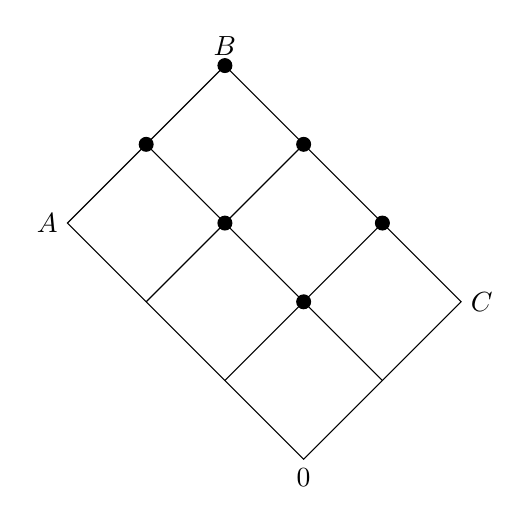
\begin{tikzpicture}[baseline={([yshift=-.5ex]current bounding box.center)}]
		\draw (-2,0) node[left] {$A$} -- (1,-3) node[below] {$0$}
		-- (3,-1) node[right] {$C$} -- (0,2) node[above] {$B$}-- cycle;
		\draw (-1,-1) -- (1,1);
		\draw (-1,1) -- (2,-2);
		\draw (0,-2) -- (2,0);
			\node[circle,draw=black, fill=black, inner sep=0pt,minimum size=5pt] at (1,1) {};
	\node[circle,draw=black, fill=black, inner sep=0pt,minimum size=5pt] at (0,2) {};
	\node[circle,draw=black, fill=black, inner sep=0pt,minimum size=5pt] at (-1,1) {};
	\node[circle,draw=black, fill=black, inner sep=0pt,minimum size=5pt] at (0,0) {};
	\node[circle,draw=black, fill=black, inner sep=0pt,minimum size=5pt] at (1,-1) {};
	\node[circle,draw=black, fill=black, inner sep=0pt,minimum size=5pt] at (2,0) {};
	\end{tikzpicture}
	\qquad \text{or}
	\qquad
	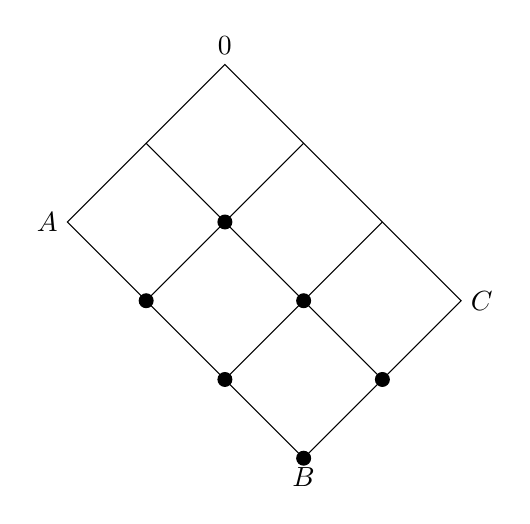
\begin{tikzpicture}[baseline={([yshift=-.5ex]current bounding box.center)}]
		\draw (-2,0) node[left] {$A$} -- (1,-3) node[below] {$B$}
		-- (3,-1) node[right] {$C$} -- (0,2) node[above] {$0$}-- cycle;
		\draw (-1,-1) -- (1,1);
		\draw (-1,1) -- (2,-2);
		\draw (0,-2) -- (2,0);
			\node[circle,draw=black, fill=black, inner sep=0pt,minimum size=5pt] at (0,0) {};
	\node[circle,draw=black, fill=black, inner sep=0pt,minimum size=5pt] at (1,-3) {};
	\node[circle,draw=black, fill=black, inner sep=0pt,minimum size=5pt] at (-1,-1) {};
	\node[circle,draw=black, fill=black, inner sep=0pt,minimum size=5pt] at (0,-2) {};
	\node[circle,draw=black, fill=black, inner sep=0pt,minimum size=5pt] at (2,-2) {};
	\node[circle,draw=black, fill=black, inner sep=0pt,minimum size=5pt] at (1,-1) {};
	\end{tikzpicture}
\end{center}
we can see that
\[
A+C-B=0.
\]
Since $A,B,C\geq 0$, the above equation force $A$ and $C$ to vanish when $B=0$. Therefore, $B$ is no longer a facet of the degeneration. Similarly, black points are all vanishing facets in the above example, and generally
the number of vanishing facets equals the number of deleted $c$s for degenerations of this type.

One can use these diamonds to build a degeneration with more vanishing facets. For example, in $A_3$
\begin{center}
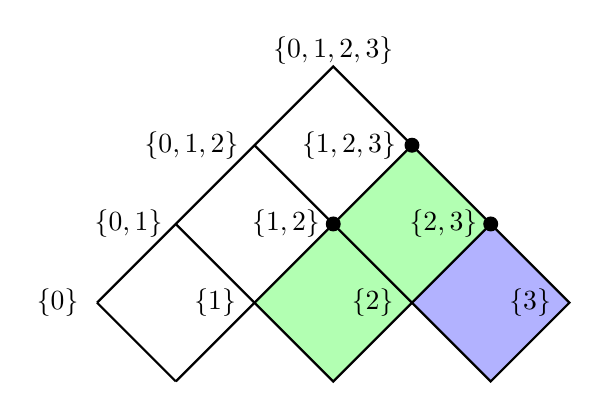
\begin{tikzpicture}
	\fill[green!30] (2,1) -- (0,-1) -- (1,-2) -- (3,0);
	\fill[blue!30] (3,0) -- (2,-1) -- (3,-2) -- (4,-1);
	\draw[thick] (-2,-1) -- (1,2) -- (4,-1) -- (3,-2) -- (0,1);
	\draw[thick] (-1,-2) -- (2,1);
	\draw[thick] (-2,-1) -- (-1,-2);
	\draw[thick] (-1,0) -- (1,-2) -- (3,0);
	\node[circle,draw=black, fill=black, inner sep=0pt,minimum size=5pt] at (1,0) {};
	\node[circle,draw=black, fill=black, inner sep=0pt,minimum size=5pt] at (2,1) {};
	\node[circle,draw=black, fill=black, inner sep=0pt,minimum size=5pt] at (3,0) {};
	\node at (-2.5,-1) {$\{0\}$};
\node at (-0.5,-1) {$\{1\}$};
\node at (1.5,-1) {$\{2\}$};
\node at (3.5,-1) {$\{3\}$};
\node at (-1.6,0) {$\{0,1\}$};
\node at (0.4,0) {$\{1,2\}$};
\node at (2.4,0) {$\{2,3\}$};
\node at (-0.8,1) {$\{0,1,2\}$};
\node at (1.2,1) {$\{1,2,3\}$};
\node at (1,2.2) {$\{0,1,2,3\}$};
\end{tikzpicture}
\end{center}
after setting $c$s in green and purple diamonds to be zero, three facets (black points) vanish and building set after deletion is 
\[
\{\{0,1,2,3\},\{0,1,2\},\{1,2,3\},\{0,1\},\{2,3\},\{0\},\{3\}\}.
\]
One can further check that it's a cube or $A_1^3$.

Suppose $\mathscr D$ is the set of all vanishing facets in the building set, 
we can read from the mesh that
\[
F_{I'}=\sum_{I\not\in \mathscr D}M_{I'}^IF_I
\]
for any $I'\in \mathscr D$, where $M$ is a matrix with non-negative entries. 
Therefore,
\[
\prod_{I\in \mathscr A_n}u_{I}^{F_{I}}=
\prod_{I'\in \mathscr D}u_{I'}^{F_{I'}}
\cdot
\prod_{I\not\in \mathscr D}u_{I}^{F_{I}}=
\prod_{I\not\in \mathscr D}\biggl(
u_I\prod_{I'\in \mathscr D}u_{I'}^{M_{I'}^I}
\bigg)^{F_I},
\]
so the new $u$-variables of the degeneration are
\[
    \tilde u_{I}=u_I\prod_{I'\in \mathscr D}u_{I'}^{M_{I'}^I}
\]
for any $I\not\in \mathscr D$. 

For example, in the above example of $A_3$,
\[
F_{123}=F_{1}+F_2+F_3, \quad F_{12}=F_1+F_2, \quad F_{23}=F_2+F_3,
\]
so the $u$-variables are
\begin{align*}
\tilde u_{1}&=u_1 u_{123} u_{12}=\frac{x_1}{x_{01}},\quad 
\tilde u_{2}=u_2 u_{123} u_{12}u_{23}=\frac{x_{2}}{x_{012}},\quad 
\tilde u_{3}=u_3u_{123}u_{23}=\frac{x_3}{x_{0123}},\\
\tilde u_{0}&=u_{0}=\frac{x_{0}}{x_{01}},\quad 
\tilde u_{01}=u_{01}=\frac{x_{01}}{x_{012}},\quad 
\tilde u_{012}=u_{012}=\frac{x_{012}}{x_{0123}},
\end{align*}
and they satisfy the following $u$-equations:
\[
	\tilde u_1+\tilde u_0=1,\quad \tilde u_2+\tilde u_{01}=1,
	\quad \tilde u_{3}+\tilde u_{012}=1.
\]

(Conjecture: they are all binary. In fact, I guess that $\tilde u_I\to 0$ is still given by $x_i\to 0$ for $i\in I$, then Chi's proof can be applied here.)

(Find those with perfect $u$-eq?)

*******************
\subsection*{Degenerations which lead to products}
In this section we provide an answer to the question of which degenerations of $A_n$ and $B_n$ give the most general products of such geometries. We begin by stating the following results about Nestohedra.

The maximal set of a building set $B_{max}$ is the set of all inclusion maximal elements of the building set $B$. A building set $B$ is connected if $B_{max}$ has a single element.

{\bf Theorem:}If $B_1, B_2,\cdots B_n$ are connected subsets of a building set $B$ then the corresponding nestohedron ${\mathscr N_B}$ is isomorphic to the product of the nestohedra ${\mathscr N}_{ B_1} \times{\mathscr N}_{ B_2} \cdots \times {\mathscr N}_{B_n}$.

We can use the above result to construct 	a degeneration of $A_n$ which is a most general product i.e., $\prod_{p_i} A_{p_i}$ such that $\sum_{i} p_{i} = n$. 

Let us consider the  $A_4$ example for which the allowed possibilities are : $A_1^{4}$, $A_1^2 \times A_2$, $A_1 \times A_3$ and $A^{2}_2$.
 
For the $A_1^{4}$ the building set is $ \{ {0},{1},{2},{3},{4},{01},{12},{23},{34} \}$ where $\{0,01\} , \{1,12\},\{2,23\},\{3,34\}$ generate the 4 $A_1$'s.

For the $A_1^{2} \times A_2$ the building set is $ \{ {0},{1},{2},{3},{4},{01},{12},{23},{34},{234} \}$ where $\{0,01\} , \{1,12\} $ generate the 2 $A_1$'s and $\{2,3,4,23,34,234\}$ generates the $A_2$'s.

For the $A_1 \times A_3$ the building set is $ \{ {0},{1},{2},{3},{4},{01},{12},{23},{34},{123},{234},{1234} \}$ where $\{0,01\}$ is the generates the $A_1$ and $\{{1},{2},{3},{4},{12},{23},{34},{123},{234},{1234} \}$ generate  $A_3$'s.

For the $A_2^{2}$ the building set is $ \{ {0},{1},{2},{3},{4},{01},{12},{23},{34} ,{012},{234}\}$ where $\{0,1,2,01,12,012\}$  and $\{2,3,4,23,34,234\}$ generate the 2 $A_2$'s.

We can similarly find a degeneration of $A_n,B_n,~or~ {\mathscr P_n}$ which would correspond to any product.







\section*{Permutahedron}
 For $x_1,x_2, \cdots, x_{n+1} \in \mathbb{R} $ , the permutahedron $P_n(x_1,\cdots,x_{n+1})$ is a convex polytope in $\mathbb{R}^{n+1}$ defined as the convex hull of all vectors obtained from $(x_1,x_2, \cdots, x_{n+1})$ by permutations of the coordinates:
 \bea
 P_n(x_1,x_2, \cdots, x_{n+1}) = ConvexHull \{ (x_{w(1)},x_{w(2)}, \cdots, x_{w(n+1)})~ |~ w \in S_{n+1} \}, \nonumber
 \eea
 where $S_{n+1}$ is the symmetric group. 
 
 The permutahedron has $(n+1)!$ vertices and is of dimension at most $n$ since it lies in the hyperplane 
 \bea
 H_c= \{(t_1,t_2, \cdots, t_{n+1}) | t_1 + t_2 + \cdots + t_{n+1}= c \} \subset \mathbb{R}^{n+1}, \nonumber
 \eea
where $c= x_1+x_2+ \cdots +x_{n+1}$

For $n=2$ and distinct $x_1,x_2, x_3$ the permutahedron $P_2(x_1,x_2, x_3)$ is a hexagon. If two of the $x_i$'s are equal then the permutahedron degenerates into a triangle and if $x_1= x_2 = x_3$ then its degenerates into a single point.

We shall state a few results about permutahedra:

{\bf Rado's theorem}: For any $x_1 \ge x_2  \cdots \ge x_{n+1}$ a point $(t_1,t_2, \cdots, t_{n+1}) \in \mathbb{R}^{n+1}$ belongs to the permutahedron $P_n(t_1,t_2, \cdots, t_{n+1})$ if and only if 
\bea
t_1+ \cdots +t_{n+1} = x_1 +\cdots+ x_{n+1} \nonumber
\eea
and for any nonemepty subset $\{i_1,\cdots,i_k \} \subset \{1,\cdots, n+1 \}$, we have 
\bea
t_{i_1}+ \cdots +t_{i_k} \leq x_1 +\cdots+ x_k \nonumber
\eea
The combinatorial structure of the permutahedron $P_n (x_1, \cdots, x_{n+1}) $ does not depend on $ x_1, \cdots, x_{n+1} $ as long as all these are distinct. 

{\bf Proposition 2}: For any  $x_1> \cdots > x_{n+1} $. The $d$-dimensional faces of $P_n ( x_1, \cdots, x_{n+1 })$ are in one-to-one correspondence with the disjoint subdivisions of the corresponding set $\{x_1,\cdots, x_{n+1 }\}$ into nonempty ordered blocks $B_1 \cup B_2 \cup \cdots \cup B_{n+1-d} =\{1,\cdots,n+1 \}$. The face corresponding to $B_1,\cdots, B_{n+1-d}$ is given by the $n+1-d$ linear equations 
\bea
\sum_{i \in B_1\cup \cdots \cup B_k} t_i = x_1 + \cdots +x_{| B_1 \cup \cdots \cup B_k |}, ~~~ for~ k=1,\cdots,n+1-d \nonumber
\eea 
\section*{Generalized permutahedra}
Generalized permutahedra are polytopes which are deformations of the usual permutahedron i.e., obtained by moving the vertices of the usual permutahedron so that the directions of all the edges are preserved though some of the edges may degenerate into points.

 Since each generalised permutahedron is obtained by parallel translation of facets of the usual permutahedron it is parametrized  by a collection $\{ z_I\}$ of $2^{n+1}-1$ coordinates, for non-empty sets of $I \subset [n+1] := \{1,\cdots,n+1 \}$
 \bea
 P_n^z(\{ z_I \}) = \left \{ (t_1, t_2, \cdots , t_{n+1}) \in \mathbb{R}^{n+1} | \sum_{i=1}^{n+1} t_i = z_{[n+1]},~ \sum_{i \in I} t_i \geq z_I, ~for ~subsets~ I  \right  \} \nonumber
 \eea
 
 If $z_I =z_J$ whenever $|I| =|J|$, then  $ P_n^z(\{ z_I \})$ is the usual permutahedron.
 
 
 A different construction of the generalised permutahedron is the following :
 
 Let, $\Delta_{[n+1]} = ConvexHull(e_1,\cdots,e_n)$ be the standard coordinate simplex in $\mathbb{R}^{n+1}$. For any $I \subset [n+1] $ let $\Delta_I =ConvexHull(e_i~|~i\in I)$ denote the face of the $\Delta_{[n+1]}$. The polytope $P_n^y(\{y_I \})$ obtained as the Minkowski sum of simplices $\Delta_I$ scaled by  parameters $y_I \geq 0$ for all nonempty subsets $I \subset [n+1]$
 \bea
 P_n^y(\{y_I \})= \sum_{I \subset[n+1]} y_I . \Delta_I  \nonumber
 \eea
is the generalised permutahedron $P_n^z(\{z_I \})$  provided $z_I = \sum_{J \subset I} y_J  ~ for ~all~nonempty ~I \subset [n+1]$.
Note that all generalised permutahedra cannot be written as Minkowski sum of coordinate simplices and we shall restrict ourselves to the large class of generalised permutahedra which admit such a realisation.
\section*{Nested Complex}
Since the combinatorial structure of the generalised permutahedron depends only on the set $B$ of nonemepty subsets $I \subset [n+1]$ such that $y_I \geq 0$ which is called the {\it building set}. We can describe the combinatorial structure when $B$ additionally satisfies the following:

\noindent(1) If $I,J \in B$ and $I \cap J \neq \phi $, then $I \cup J \in B$. \\
(2) $B$ contains all singletons $\{ i\}$ for $i \in S$.

A subset $N$ in the building set $B$ is called a {\it nested set} if it satisfies the following conditions:\\
\noindent
(1) For any $I,J \in N$, we either have $I \subset J$ or $J\subset I$ or $I$ and $J$ are disjoint.\\
(2) For any collection of $k \geq 2$ disjoint subsets $J_1,J_2,\cdots, J_k \in N$ their union $J_1 \cup \cdots \cup J_k$ is not in B. \\
(3) N contains all maximal elements of $B$.

The {\it nested complex} $\mathcal{N}(B)$ is defined as the poset of the set of all nested sets in $B$ ordered by inclusion.

{\bf Theorem 1}: Let us assume that the set $B$ associated with a generalised permutahedron $P_n^{y}$ is a building set on $[n+1]$. Then the poset of faces $P_n^{y}$ ordered by reverse inclusion is isomorphic to the nested complex $\mathcal{N}(B)$. 

{\bf Theorem 2}: Let us assume that the set $B$ associated with a generalised permutahedron $P_n^{y}$ is a building set on $[n+1]$. The face $P_N$ of $P_n^{y}(y_I)$ associated with the nested set $N \in \mathcal{N}(B)$ is given by:
\bea
P_N = \left \{ \right (t_1,\cdots,t_{n+1}) \in \mathbb{R}^{n+1} | \sum_{i \in I} t_i =y_{I}~for~I \in N; ~ \sum_{i \in J}t_i \geq y_J, for J \in B  )\}
\eea
In particular the dimension of the face $P_N$ equals $n+1-|N|$. 

In summary the above results imply that we can look at any collection of subsets of $[n+1]$ which form a building set $B$ and associate  coordinate simplex $\Delta_I$ for each $I \in B$ and resulting Minkowski sum with positive weights $y_I$ generates a generalised permutahedron associated with the building set. Further, the number of facets of the generalised permutahedron just correspond to the set of all non-singlet elements in $B$.  
We shall use $ \{0,1,\cdots,n \}$ instead of $[n+1]$ with $x_0 =1$ from now on. Since, the number of singlets correspond to the dimension of the generalised permutahedron this implies that:

{\bf Number of facets = Number of linear equation + dimension of  gen permutahedron}
 
Thus, generalised permutahedra have "Big Polytope" which correspond to a simplex and we can write down the stringy canonical forms and solve for the $u$-variables and examine if they satisfy some kind of $u$-equations.

Here are some interesting examples of generalised permutahedra:

(1) If $B$ consists of only singlets i.e., $B=\{ \{ 0,1,\cdots,n \}, \{ 0 \},\{ 1 \},\cdots ,\{ n \} \}$ then the generalised permutahedron is a Simplex. In this case the relevant $x$ variables are $x_i,~ i=0,\cdots,n$ and $\sum_{i=0}^n x_i$. 
The Newton polytope of the Minkowski sum is $\prod_{i=1}^{n} x_i (1+\sum_{j=1}^{n} x_j)$ and $u$-variables are 
$u_i =\frac{ x_i}{1+\sum_{i=1}^n x_i} $
which satisfy $\sum u_i =1$ as their only $u$-equation. \\

(2) If $B= \{[i] | i=1,\cdots,n+1 \}$ is the complete flag of intervals, then $P_n({\bf Y})$ is the Stanley-Pitman polytope or Hypercube.
The Newton polytope of the Minkowski sum is $x_1\cdots x_n (1+x_1) \cdots (1+x_1+\cdots +x_n)$ and $u$-variables are 
$u_i =\frac{ 1}{1+\sum_{j=1}^{i} x_j} $, ~~$u^{'}_i =\frac{ \sum_{j=1}^{i} x_j}{1+\sum_{j=1}^{i} x_j} $ for $j=1,\cdots,n$ \\
which satisfy $u_i +u^{'}_{i} =1$ as their $u$-equation. \\

(3) If $B$ corresponds to all the non empty subsets of $\{0,1,\cdots,n \}$ and $Y_I =y_{|I|}$ i.e., the variables $Y_I$ are equal for all subsets of the same cardinality, then $P_n({\bf Y})$ is the usual permutahedron $P_n$. 

\section*{ABHY like realisation for the Permutahedron}
The following set of equations to define the $n$-dimensional Permutahedron: 
\bea
C_I = (-1)^{|I|} \left( \sum_{i \in I} X_i - \sum _{{i<j}\atop{i,j \in I}} X_{ij} +\cdots + (-1)^{|I|}  X_I \right) \nonumber
\eea
for all non-empty subsets $I \subset \{0,1,\cdots,n\}$ with the understanding that $C_{I} =0$ for all singlets $I$ and $X_{I} =0$ for $I=\{ 0,1,\cdots,n \}$. 

It is clear that
\bea
m= \text{No. of  C's }&=& 2^{n+1}-(n+2) \nonumber \\
N= \text{No. of X's} &=& 2^{n+1}- 2 \nonumber 
\eea
Thus we see that $N= d+m$ and hence the "Big polytope" in this case is again a simplex. We can write down the stringy integral as usual to be 
\bea
\int_{\mathbb{R}^{n}_{+}} \prod_{i =1}^{n} d x_i x_i^{\alpha^{'} X_i -1} \prod_{I} \left (\sum_{a\in I} x_a \right) ^{-\alpha^{'} C_I} \nonumber
\eea 
where the product is over all non-singlets $ I \subset \{0,1,\cdots,n\}$ with $x_{0} =1$.

We can then solve for the corresponding $u's$ :
\bea
u_J &=& ~~\prod_{J \subset I} x_I^{(-1)^{|I|-|J|}} \nonumber \\
u^{'}_J &=& \prod_{{0 \in I}\atop{ \{0,\cdots,n\} - I \subset J}} x_I^{(-1)^{|I|-|J|+\color{red}{mod(n, 2)}}} \nonumber
\eea

\section*{2d permutahedron}
In this case the building set $B=\{ \{ 0,1,2\},\{ 0,1\},\{0,2\},\{1,2\},\{0\},\{1\},\{2\}\}$ and the relevant $x$ variables are $x_0=1, ~x_1=x, ~x_2=y, ~x_{01}=1+x, ~x_{02}=1+y,~ x_{12}=x+y,~ x_{012}=1+x+y$. 

We can write down the Newton polynomial for the Minkowski sum as $ x_1~ x_2~(1+x_1)~(1+x_2)~(x_1+x_2)~(1+x_1+x_2)$.

The $u$-variables can be written in terms of $x$ variables as:
\bea
u_1&=&\frac{x(1+x+y)}{(x+y)(1+x)}, ~ u_2 =\frac{y(1+x+y)}{(x+y)(1+y)},~ u_{12}=\frac{(x+y)}{(1+x+y)}\nonumber \\
u^{'}_1&=&\frac{(1+y)}{(1+x+y)}, ~~~~~ u^{'}_2=\frac{(1+x)}{(1+x+y)},~~~~~ u^{'}_{12}= \frac{(1+x+y)}{(1+x)(1+y)} \nonumber
\eea
The $u$-equations are:
\bea
1-u_i &=& (u^{'}_i)^2 u_j u^{'}_{12}, ~~~ 1-u_{12} = u^{'}_{1} u^{'}_{2} u^{'}_{12} \nonumber \\
1-u^{'}_i &=& u_i u^{'}_j u_{12}, ~~~~~~~ 1-u^{'}_{12} = u_{1} u_{2} (u_{12})^2 \nonumber
\eea
where $i=1$ implies $j=2$ and vice versa.
Let us look at the $n=3$ example.

\section*{3d permutahedron}
In this case the building set $B=\{ \{ 0,1,2,3\},\{ 0,1,2\},\{0,2,3\},\{0,1,3\},\{1,2,3\},\{0,1\},\{0,2\},\{0,3\},\{1,2\} \\ ,\{2,3\},\{1,3\},\{0\},\{1\},\{2\},\{3\}\}$ and the relevant $x$ variables are $x_0=1, ~x_1=x, ~x_2=y, ~x_3=z, ~x_{01}=1+x, ~x_{02}=1+y,~x_{03}=1+z,~ x_{12}=x+y,~x_{13}=x+z,~x_{23}=y+z,~ x_{012}=1+x+y,~ x_{013}=1+x+z,~ x_{023}=1+y+z,~ x_{123}=x+y+z,~ x_{0123}=1+x+y+z$. \\

The $u$ and $u'$-variables can be written interms of $x$ variables as:
{\scriptsize  \bea
u_1&=&\frac{x(1+x+y)(1+x+z)(x+y+z)}{(x+y)(x+z)(1+x)(1+x+y+z)}, ~ u_2 =\frac{y(1+x+y)(1+y+z)(x+y+z)}{(x+y)(y+z)(1+y)(1+x+y+z)},~ u_{3}=\frac{z(1+x+z)(1+y+z)(x+y+z)}{(x+z)(y+z)(1+z)(1+x+y+z)},\nonumber \\
u^{'}_1&=&\frac{(1+y+z)}{(1+x+y+z)}, ~~~~~~~~~~~~~~~~~~~~~~~~~~~~ u^{'}_2 =\frac{(1+x+z)}{(1+x+y+z)},~~~~~~~~~~~~~~~~~~~~~~~~~~~~~ u^{'}_{3}=\frac{(1+x+y)}{(1+x+y+z)},\nonumber \\
u_{12}&=&\frac{(x+y)(1+x+y+z)}{(1+x+y)(x+y+z)}, ~~~~~~~~~~~~~~~~~~ u_{23} =\frac{(y+z)(1+x+y+z)}{(1+y+z)(x+y+z)},~~~~~~~~~~~~~~~~~~~ u_{13}=\frac{(x+z)(1+x+y+z)}{(1+x+z)(x+y+z)},\nonumber \\
u^{'}_{12}&=&\frac{(1+z)(1+x+y+z)}{(1+y+z)(1+x+z)}, ~~~~~~~~~~~~~~~~~~ u^{'}_{23} =\frac{(1+x)(1+x+y+z)}{(1+x+y)(1+x+z)},~~~~~~~~~~~~~~~~~~~ u^{'}_{13}=\frac{(1+y)(1+x+y+z)}{(1+x+y))(1+y+z)},\nonumber  \\
u_{123}&=&\frac{(x+y+z)}{(1+x+y+z)}, ~~~~~~~~~~~~~~~~~~~~~~~~~~~ u^{'}_{123} =\frac{(1+x+y)(1+y+z)}{(1+x)(1+y)(1+z)(1+x+y+z)}\nonumber
\eea }
The $u$-equations in this case are:
{\small  \bea
1-u_i &=& u_j u_k (u_{jk})^2 (u^{'}_i)^3 (u^{'}_{ij})^2(u^{'}_{ik})^2 u^{'}_{123} \left(1+ u_i u_{ij} u_{ik} u^{'}_{j} u^{'}_{k}  u^{'}_{jk}\right), ~~ 1-u_{ij} = u_k u_{ik} u_{jk} (u^{'}_i)^2 (u^{'}_{j})^2 (u^{'}_{ij})^2 u^{'}_{ik} u^{'}_{jk} u^{'}_{123} \nonumber  \\
1-u^{'}_i &=& u_i u_{ij} u_{ik} u^{'}_{j} u^{'}_{k}  u^{'}_{jk}, ~~~~~~~~~~~~~~~~~~~~~~~~~~~~~~~~~~~~~~~~~~~~~~~~~~~~~ 1-u^{'}_{ij} = u_i u_{j}  (u_{ij})^2 u_{ik} u_{jk} (u_{123})^2 (u^{'}_{k})^2 u^{'}_{ik} u^{'}_{jk}  \nonumber \\
1-u^{'}_{123} &=& u_1 u_{2} u_{3} (u_{12})^2 (u_{23})^2  (u_{13})^2 (u_{123})^3 \left(1+ u^{'}_{123}  u^{'}_1 u^{'}_{2} u^{'}_{3} u^{'}_{12} u^{'}_{23}  u^{'}_{13} \right), 1-u_{123} = u^{'}_1 u^{'}_{2} u^{'}_{3} u^{'}_{12} u^{'}_{23}  u^{'}_{13} u^{'}_{123}   \nonumber
\eea}
where $i,j,k \in {1,2,3}$ and $i \neq j \neq k$.

The 8 facets of the 3d permutahedron corresponding to $u_i \rightarrow 0, u^{'}_i \rightarrow 0,u_{123} \rightarrow 0 ~and ~u^{'}_{123} \rightarrow 0$  are all $B_2$'s. Similarly, the 6 facets corresponding to  $u_{ij} \rightarrow 0, u^{'}_{ij} \rightarrow 0$ are all  $A^{2}_1$.

Thus, the 3d permutahedron integral factorizes nicely on all massless poles at finite $\alpha^{'}$ !!
\section*{4d permutahedron}
The $u$ variables for the 4d permutahedron are:
{\tiny
\begin{align*}
u_1&= \frac{x (w+x+1) (x+y+1) (w+x+y) (x+z+1) (w+x+z)
   (x+y+z) (w+x+y+z+1)}{(x+1) (w+x) (x+y) (w+x+y+1) (x+z) (w+x+z+1) (x+y+z+1)
   (w+x+y+z)},\nonumber \\  u_2 &= \frac{y (w+y+1) (x+y+1) (w+x+y) (y+z+1) (w+y+z) (x+y+z)
   (w+x+y+z+1)}{(y+1) (w+y) (x+y) (w+x+y+1) (y+z) (w+y+z+1) (x+y+z+1)
   (w+x+y+z)} \nonumber \\  u_3 &= \frac{z (w+z+1) (x+z+1) (w+x+z) (y+z+1) (w+y+z) (x+y+z)
   (w+x+y+z+1)}{(z+1) (w+z) (x+z) (w+x+z+1) (y+z) (w+y+z+1) (x+y+z+1)
   (w+x+y+z)},\nonumber \\ u_4 &= \frac{w (w+x+1) (w+y+1) (w+x+y) (w+z+1) (w+x+z) (w+y+z) (w+x+y+z+1)}{(w+1)
   (w+x) (w+y) (w+x+y+1) (w+z) (w+x+z+1) (w+y+z+1) (w+x+y+z)},\nonumber \\
   u_{12} &=  \frac{(x+y) (w+x+y+1) (x+y+z+1) (w+x+y+z)}{(x+y+1) (w+x+y)
   (x+y+z) (w+x+y+z+1)},~u_{13} = \frac{(x+z) (w+x+z+1) (x+y+z+1) (w+x+y+z)}{(x+z+1) (w+x+z)
   (x+y+z) (w+x+y+z+1)},\nonumber \\ ~ u_{14} &= \frac{(w+x)(w+x+y+1) (w+x+z+1) (w+x+y+z)}{(w+x+1) (w+x+y) (w+x+z) (w+x+y+z+1)}, u_{24} = \frac{(w+y) (w+x+y+1) (w+y+z+1) (w+x+y+z)}{(w+y+1) (w+x+y) (w+y+z) (w+x+y+z+1)},\nonumber \\ ~u_{23} &=
   \frac{(y+z) (w+y+z+1) (x+y+z+1) (w+x+y+z)}{(y+z+1) (w+y+z) (x+y+z)(w+x+y+z+1)},~ u_{34} = \frac{(w+z) (w+x+z+1) (w+y+z+1) (w+x+y+z)}{(w+z+1) (w+x+z) (w+y+z) (w+x+y+z+1)}, \nonumber \\  
  u_{123} &= \frac{(x+y+z) (w+x+y+z+1)}{(x+y+z+1)(w+x+y+z)},~u_{134}= \frac{(w+x+z) (w+x+y+z+1)}{(w+x+z+1)(w+x+y+z)},~ u_{124}= \frac{(w+x+y) (w+x+y+z+1)}{(w+x+y+1) (w+x+y+z)},~ u_{234} = \frac{(w+y+z) (w+x+y+z+1)}{(w+y+z+1) (w+x+y+z)},\nonumber \\
    u_{1234} &= \frac{w+x+y+z}{w+x+y+z+1},\nonumber \\ u'_1&= \frac{w+y+z+1}{w+x+y+z+1},~~u'_2= \frac{w+x+z+1}{w+x+y+z+1}, u'_3=  \frac{w+x+y+1}{w+x+y+z+1},u'_4 = \frac{x+y+z+1}{w+x+y+z+1}, \nonumber \\  u'_{12} &= \frac{(w+z+1) (w+x+y+z+1)}{(w+x+z+1) (w+y+z+1)}, u'_{13} = \frac{(w+y+1) (w+x+y+z+1)}{(w+x+y+1) (w+y+z+1)},\nonumber \\  u'_{14} &= \frac{(y+z+1) (w+x+y+z+1)}{(w+y+z+1) (x+y+z+1)},u'_{23} = \frac{(w+x+1) (w+x+y+z+1)}{(w+x+y+1) (w+x+z+1)}, \nonumber \\ u'_{24}&= \frac{(x+z+1) (w+x+y+z+1)}{(w+x+z+1)(x+y+z+1)}, u'_{34}=  \frac{(x+y+1) (w+x+y+z+1)}{(w+x+y+1) (x+y+z+1)},\nonumber \\  
u'_{123} &=  \frac{(w+1) (w+x+y+1) (w+x+z+1) (w+y+z+1)}{(w+x+1) (w+y+1) (w+z+1) (w+x+y+z+1)},~u'_{124}= \frac{(z+1) (w+x+z+1) (w+y+z+1) (x+y+z+1)}{(w+z+1) (x+z+1) (y+z+1) (w+x+y+z+1)},\nonumber \\  u'_{134}&= \frac{(y+1) (w+x+y+1) (w+y+z+1) (x+y+z+1)}{(w+y+1)(x+y+1) (y+z+1) (w+x+y+z+1)},u'_{234} = \frac{(x+1) (w+x+y+1) (w+x+z+1) (x+y+z+1)}{(w+x+1) (x+y+1) (x+z+1) (w+x+y+z+1)},\nonumber \\  u'_{1234} &= \frac{(w+x+1) (w+y+1)(x+y+1) (w+z+1) (x+z+1) (y+z+1) (w+x+y+z+1)}{(w+1) (x+1) (y+1) (w+x+y+1) (z+1) (w+x+z+1) (w+y+z+1) (x+y+z+1)} \nonumber
\end{align*}
}
\newpage
\vspace*{-25pt}
The $u$ equations are 
{\tiny
{\begin{align*}
1-u_1&=u_2 u_3 u_4 u_{2,3}^2 u_{24}^2 u_{34}^2 u_{234}^4
   \left(u'\right)_1^8 \left(u'\right)_{12}^4 \left(u'\right)_{13}^4
   \left(u'\right)_{14}^4 \left(u'\right)_{123}^2
   \left(u'\right)_{124}^2 \left(u'\right)_{134}^2 u'_{1234}+ 6~
 \textcolor{red}{  u_1^2} u_2 u_3 u_4 u_{12}^2 u_{13}^2 u_{14}^2 u_{23}^2 u_{24}^2
   u_{34}^2 u_{123}^2 u_{124}^2 u_{134}^2 u_{234}^3 u_{1234}
   u'_2 u'_3 u'_4 \left(u'\right)_1^4  \nonumber \\ &\left(u'\right)_{12}^3
   \left(u'\right)_{13}^3 \left(u'\right)_{14}^3
   \left(u'\right)_{23}^2 \left(u'\right)_{24}^2
   \left(u'\right)_{34}^2 \left(u'\right)_{123}^2
   \left(u'\right)_{124}^2 \left(u'\right)_{134}^2
   \left(u'\right)_{234}^2 u'_{1234}+~2 ~\textcolor{red}{u_1} u_2 u_3 u_4 u_{12}
   u_{13} u_{14} u_{23}^2 u_{24}^2 u_{34}^2 u_{123} u_{124}
   u_{134} u_{234}^3 \left(u'\right)_1^4 \left(u'\right)_{12}^3
   \left(u'\right)_{13}^3 \nonumber \\ & \left(u'\right)_{14}^3 u'_{23} u'_{24}
   u'_{34} \left(u'\right)_{123}^2 \left(u'\right)_{124}^2
   \left(u'\right)_{134}^2 u'_{234} \left(u_{234}
   \left(1-u_{1234}\right) u_{1234} u'_1+u'_2 u'_3
   \left(1-u'_{23}\right)+u'_2 u'_4 \left(1-u'_{24}\right)+u'_3 u'_4
   \left(1-u'_{34}\right)+\left(u'\right)_1^2\right) u'_{1234} ,\nonumber \\
   1-u_2&=u_1 u_3 u_4 u_{13}^2 u_{14}^2 u_{34}^2 u_{134}^4
   \left(u'\right)_2^8 \left(u'\right)_{12}^4 \left(u'\right)_{23}^4
   \left(u'\right)_{24}^4 \left(u'\right)_{123}^2
   \left(u'\right)_{124}^2 \left(u'\right)_{234}^2 u'_{1234}+~6
   u_1 \textcolor{red}{u_2^2} u_3 u_4 u_{1,2}^2 u_{13}^2 u_{14}^2 u_{23}^2 u_{24}^2
   u_{34}^2 u_{123}^2 u_{124}^2 u_{134}^3 u_{234}^2 u_{1234}
   u'_1 u'_3 u'_4 \left(u'\right)_2^4 \nonumber \\ &\left(u'\right)_{12}^3
   \left(u'\right)_{13}^2 \left(u'\right)_{14}^2
   \left(u'\right)_{23}^3 \left(u'\right)_{24}^3
   \left(u'\right)_{34}^2 \left(u'\right)_{123}^2
   \left(u'\right)_{124}^2 \left(u'\right)_{134}^2
   \left(u'\right)_{234}^2 u'_{1234}+~2~ u_1 \textcolor{red}{u_2} u_3 u_4 u_{12}
   u_{13}^2 u_{14}^2 u_{23} u_{24} u_{34}^2 u_{123} u_{124}
   u_{134}^3 u_{234} \left(u'\right)_2^4 \left(u'\right)_{12}^3
   u'_{13} u'_{14} \nonumber \\ & \left(u'\right)_{23}^3 \left(u'\right)_{24}^3
   u'_{34} \left(u'\right)_{123}^2 \left(u'\right)_{124}^2
   u'_{134} \left(u'\right)_{234}^2 \left(u_{134}
   \left(1-u_{1234}\right) u_{1234} u'_2+u'_1 u'_3
   \left(1-u'_{13}\right)+u'_1 u'_4 \left(1-u'_{14}\right)+u'_3 u'_4
   \left(1-u'_{34}\right)+\left(u'\right)_2^2\right) u'_{1234} ,\nonumber \\
   1-u_3&=u_1 u_2 u_4 u_{12}^2 u_{14}^2 u_{24}^2 u_{124}^4
   \left(u'\right)_3^8 \left(u'\right)_{13}^4 \left(u'\right)_{23}^4
   \left(u'\right)_{34}^4 \left(u'\right)_{123}^2
   \left(u'\right)_{134}^2 \left(u'\right)_{234}^2 u'_{1234}+~6
   u_1 u_2 \textcolor{red}{u_3^2} u_4 u_{12}^2 u_{13}^2 u_{14}^2 u_{23}^2 u_{24}^2
   u_{34}^2 u_{123}^2 u_{124}^3 u_{134}^2 u_{234}^2 u_{1234}
   u'_1 u'_2 u'_4 \left(u'\right)_3^4 \nonumber \\ & \left(u'\right)_{12}^2
   \left(u'\right)_{13}^3 \left(u'\right)_{14}^2
   \left(u'\right)_{23}^3 \left(u'\right)_{24}^2
   \left(u'\right)_{34}^3 \left(u'\right)_{123}^2
   \left(u'\right)_{124}^2 \left(u'\right)_{134}^2
   \left(u'\right)_{234}^2 u'_{1234} +~2 ~u_1 u_2 \textcolor{red}{u_3} u_4 u_{1,2}^2
   u_{13} u_{14}^2 u_{23} u_{24}^2 u_{34} u_{123} u_{124}^3
   u_{134} u_{234} \left(u'\right)_3^4 u'_{12}
   \left(u'\right)_{13}^3 u'_{14} \nonumber \\ &\left(u'\right)_{23}^3 u'_{24}
   \left(u'\right)_{34}^3 \left(u'\right)_{123}^2 u'_{124}
   \left(u'\right)_{134}^2 \left(u'\right)_{234}^2 \left(u_{124}
   \left(1-u_{1234}\right) u_{1234} u'_3+u'_1 u'_2
   \left(1-u'_{12}\right)+u'_1 u'_4 \left(1-u'_{14}\right)+u'_2 u'_4
   \left(1-u'_{24}\right)+\left(u'\right)_3^2\right) u'_{1234} ,\nonumber \\
   1-u_4 &= u_1 u_2 u_3 u_{12}^2 u_{13}^2 u_{23}^2 u_{123}^4
   \left(u'\right)_4^8 \left(u'\right)_{14}^4 \left(u'\right)_{24}^4
   \left(u'\right)_{34}^4 \left(u'\right)_{124}^2
   \left(u'\right)_{134}^2 \left(u'\right)_{234}^2 u'_{1234}+~6
   u_1 u_2 u_3 \textcolor{red}{u_4^2} u_{12}^2 u_{13}^2 u_{14}^2 u_{23}^2 u_{24}^2
   u_{34}^2 u_{123}^3 u_{124}^2 u_{134}^2 u_{234}^2 u_{1234}
   u'_1 u'_2 u'_3 \left(u'\right)_4^4 \nonumber\\ &\left(u'\right)_{12}^2
   \left(u'\right)_{13}^2 \left(u'\right)_{14}^3
   \left(u'\right)_{23}^2 \left(u'\right)_{24}^3
   \left(u'\right)_{34}^3 \left(u'\right)_{123}^2
   \left(u'\right)_{124}^2 \left(u'\right)_{134}^2
   \left(u'\right)_{234}^2 u'_{1234}+~2 u_1 u_2 u_3 \textcolor{red}{u_4} u_{12}^2
   u_{13}^2 u_{14} u_{23}^2 u_{24} u_{34} u_{123}^3 u_{124}
   u_{134} u_{234} \left(u'\right)_4^4 u'_{12} u'_{13}
   \left(u'\right)_{14}^3 \nonumber\\ &u'_{23} \left(u'\right)_{24}^3
   \left(u'\right)_{34}^3 u'_{123} \left(u'\right)_{124}^2
   \left(u'\right)_{134}^2 \left(u'\right)_{234}^2 \left(u_{123}
   \left(1-u_{1234}\right) u_{1234} u'_4+u'_1 u'_2
   \left(1-u'_{12}\right)+u'_1 u'_3 \left(1-u'_{13}\right)+u'_2 u'_3
   \left(1-u'_{23}\right)+\left(u'\right)_4^2\right) u'_{1234},\nonumber \\
    1-u_{12}&= u_3 u_4
   u_{13} u_{14} u_{23} u_{24} u_{34}^2 u_{134}^2 u_{234}^2 \left(u'\right)_1^3
   \left(u'\right)_2^3 \left(u'\right)_{12}^3 \left(u'\right)_{13}^2
   \left(u'\right)_{14}^2 \left( u'\right)_{23}^2 \left(u'\right)_{24}^2 \left(1+u_{12}
   u_{123} u_{124} u_{1234} u'_3 u'_4 u'_{34}\right) \left(u'\right)_{123}^2
   \left(u'\right)_{124}^2 u'_{134} u'_{234} u'_{1234},\nonumber \\
     1-u_{13}&=u_2 u_4 u_{12}
   u_{14} u_{23} u_{24}^2 u_{34} u_{124}^2 u_{234}^2 \left(u'\right)_1^3
   \left(u'\right)_3^3 \left(u'\right)_{12}^2 \left(u'\right)_{13}^3
   \left(u'\right)_{14}^2 \left(u'\right)_{23}^2 \left(1+ u_{13} u_{123} u_{134} u_{1234}
   u'_2 u'_4 u'_{24}\right) \left(u'\right)_{34}^2 \left(u'\right)_{123}^2 u'_{124}
   \left(u'\right)_{134}^2 u'_{234} u'_{1234},\nonumber \\ 
   1-u_{14}&= u_2 u_3 u_{12} u_{13} u_{23}^2 u_{24} u_{34} u_{123}^2 u_{234}^2
   \left(u'\right)_1^3 \left(u'\right)_4^3 \left(u'\right)_{12}^2 \left(u'\right)_{13}^2
   \left(u'\right)_{14}^3 \left(1+ u_{14} u_{124} u_{134} u_{1234} u'_2 u'_3
   u'_{23}\right) \left(u'\right)_{24}^2 \left(u'\right)_{34}^2 u'_{123}
   \left(u'\right)_{124}^2 \left(u'\right)_{134}^2 u'_{234} u'_{1234}, \nonumber \\ 
    1-u_{34}&= u_1 u_2 u_{12}^2 u_{13}
   u_{14} u_{23} u_{24} u_{123}^2 u_{124}^2 \left(u'\right)_3^3 \left(u'\right)_4^3
   \left(1+u_{34} u_{134} u_{234} u_{1234} u'_1 u'_2 u'_{12}\right)
   \left(u'\right)_{13}^2 \left(u'\right)_{14}^2 \left(u'\right)_{23}^2
   \left(u'\right)_{24}^2 \left(u'\right)_{34}^3 u'_{123} u'_{124}
   \left(u'\right)_{134}^2 \left(u'\right)_{234}^2 u'_{1234}, \nonumber \\ 
   1-u_{24}&=u_1 u_3 u_{12} u_{13}^2 u_{14}
   u_{23} u_{34} u_{123}^2 u_{134}^2 \left(u'\right)_2^3 \left(u'\right)_4^3
   \left(u'\right)_{12}^2 \left(1+ u_{24} u_{124} u_{234} u_{1234} u'_1 u'_3
   u'_{13}\right) \left(u'\right)_{14}^2 \left(u'\right)_{23}^2 \left(u'\right)_{24}^3
   \left(u'\right)_{34}^2 u'_{123} \left(u'\right)_{124}^2 u'_{134}
   \left(u'\right)_{234}^2 u'_{1234},\nonumber \\
    1-u_{23}&=u_1 u_4 u_{12} u_{13} u_{14}^2 u_{24}
   u_{34} u_{124}^2 u_{134}^2 \left(u'\right)_2^3 \left(u'\right)_3^3
   \left(u'\right)_{12}^2 \left(u'\right)_{13}^2 \left(1+u_{23} u_{123} u_{234} u_{1234}
   u'_1 u'_4 u'_{14}\right) \left(u'\right)_{23}^3 \left(u'\right)_{24}^2
   \left(u'\right)_{34}^2 \left(u'\right)_{123}^2 u'_{124} u'_{134}
   \left(u'\right)_{234}^2 u'_{1234},\nonumber \\ 
   1-u_{124}&=u_3 u_{13} u_{23} u_{34} u_{123} u_{134}
   u_{234} \left(u'\right)_1^2 \left(u'\right)_2^2 \left(u'\right)_4^2
   \left(u'\right)_{12}^2 u'_{13} \left(u'\right)_{14}^2 u'_{23} \left(u'\right)_{24}^2
   u'_{34} u'_{123} \left(u'\right)_{124}^2 u'_{134} u'_{234} u'_{1234},\nonumber \\ 
   1-u_{123}&=u_4 u_{14}
   u_{24} u_{34} u_{124} u_{134} u_{234} \left(u'\right)_1^2 \left(u'\right)_2^2
   \left(u'\right)_3^2 \left(u'\right)_{12}^2 \left(u'\right)_{13}^2 u'_{14}
   \left(u'\right)_{23}^2 u'_{24} u'_{34} \left(u'\right)_{123}^2 u'_{124} u'_{134}
   u'_{234} u'_{1234},\nonumber \\ 
   1-u_{134}&=u_2 u_{12} u_{23} u_{24} u_{123} u_{124} u_{234}
   \left(u'\right)_1^2 \left(u'\right)_3^2 \left(u'\right)_4^2 u'_{12}
   \left(u'\right)_{13}^2 \left(u'\right)_{14}^2 u'_{23} u'_{24} \left(u'\right)_{34}^2
   u'_{123} u'_{124} \left(u'\right)_{134}^2 u'_{234} u'_{1234},\nonumber \\ 
   1-u_{234}&=u_1 u_{12} u_{13} u_{14} u_{123} u_{124} u_{134}
   \left(u'\right)_2^2 \left(u'\right)_3^2 \left(u'\right)_4^2 u'_{12} u'_{13} u'_{14}
   \left(u'\right)_{23}^2 \left(u'\right)_{24}^2 \left(u'\right)_{34}^2 u'_{123} u'_{124}
   u'_{134} \left(u'\right)_{234}^2 u'_{1234},\nonumber \\ 
   1-u_{1234}&=u'_1
   u'_2 u'_3 u'_4 u'_{12} u'_{13} u'_{14} u'_{23} u'_{24} u'_{34} u'_{123} u'_{124}
   u'_{134} u'_{234} u'_{1234},\nonumber \\ 
   1-u'_1&=u_1 u_{12} u_{13} u_{14} u_{123}
   u_{124} u_{134} u_{1234} u'_2 u'_3 u'_4 u'_{23} u'_{24} u'_{34} u'_{234},\nonumber \\ 
   1-u'_2&=u_2
   u_{12} u_{23} u_{24} u_{123} u_{124} u_{234} u_{1234} u'_1 u'_3 u'_4 u'_{13} u'_{14}
   u'_{34} u'_{134},\nonumber \\ 
   1-u'_3&=u_3 u_{13} u_{23} u_{34} u_{123} u_{134} u_{234} u_{1234} u'_1
   u'_2 u'_4 u'_{12} u'_{14} u'_{24} u'_{124},\nonumber \\ 
   1-u'_4&=u_4 u_{14} u_{24} u_{34} u_{124}
   u_{134} u_{234} u_{1234} u'_1 u'_2 u'_3 u'_{12} u'_{13} u'_{23} u'_{123},\nonumber \\ 
   1-u'_{12}&=u_1
   u_2 u_{12}^2 u_{13} u_{14} u_{23} u_{24} u_{123}^2 u_{124}^2 u_{134} u_{234}
   u_{1234}^2 \left(u'\right)_3^2 \left(u'\right)_4^2 u'_{13} u'_{14} u'_{23} u'_{24}
   \left(u'\right)_{34}^2 u'_{134} u'_{234},\nonumber \\
   1-u'_{13}&=u_1 u_3 u_{12} u_{13}^2 u_{14}
   u_{23} u_{34} u_{123}^2 u_{124} u_{134}^2 u_{234} u_{1234}^2 \left(u'\right)_2^2
   \left(u'\right)_4^2 u'_{12} u'_{14} u'_{23} \left(u'\right)_{24}^2 u'_{34} u'_{124}
   u'_{234},\nonumber \\
   1-u'_{14}&=u_1 u_4 u_{12} u_{13} u_{14}^2 u_{24} u_{34} u_{123} u_{124}^2
   u_{134}^2 u_{234} u_{1234}^2 \left(u'\right)_2^2 \left(u'\right)_3^2 u'_{12} u'_{13}
   \left(u'\right)_{23}^2 u'_{24} u'_{34} u'_{123} u'_{234},\nonumber \\ 1-u'_{23}&=u_2 u_3 u_{12}
   u_{13} u_{23}^2 u_{24} u_{34} u_{123}^2 u_{124} u_{134} u_{234}^2 u_{1234}^2
   \left(u'\right)_1^2 \left(u'\right)_4^2 u'_{12} u'_{13} \left(u'\right)_{14}^2 u'_{24}
   u'_{34} u'_{124} u'_{134},\nonumber \\ 1-u'_{24}&=u_2 u_4 u_{12} u_{14} u_{23} u_{24}^2 u_{34}
   u_{123} u_{124}^2 u_{134} u_{234}^2 u_{1234}^2 \left(u'\right)_1^2 \left(u'\right)_3^2
   u'_{12} \left(u'\right)_{13}^2 u'_{14} u'_{23} u'_{34} u'_{123} u'_{134},\nonumber \\ 1-u'_{34}&=u_3
   u_4 u_{13} u_{14} u_{23} u_{24} u_{34}^2 u_{123} u_{124} u_{134}^2 u_{234}^2
   u_{1234}^2 \left(u'\right)_1^2 \left(u'\right)_2^2 \left(u'\right)_{12}^2 u'_{13}
   u'_{14} u'_{23} u'_{24} u'_{123} u'_{124},\nonumber \\
   1-u'_{123}&=u_1 u_2 u_3 u_{12}^2 u_{13}^2
   u_{14} u_{23}^2 u_{24} u_{34} u_{123}^3 u_{124}^2 u_{134}^2 u_{234}^2 u_{1234}^3
   \left(u'\right)_4^3 \left(u'\right)_{14}^2 \left(u'\right)_{24}^2
   \left(u'\right)_{34}^2 \left(1+ u'_1 u'_2 u'_3 u'_{12} u'_{13} u'_{23} u'_{123}\right)
   u'_{124} u'_{134} u'_{234},\nonumber \\ 
   1-u'_{124}&=u_1 u_2 u_4 u_{12}^2 u_{13} u_{14}^2 u_{23}
   u_{24}^2 u_{34} u_{123}^2 u_{124}^3 u_{134}^2 u_{234}^2 u_{1234}^3 \left(u'\right)_3^3
   \left(u'\right)_{13}^2 \left(u'\right)_{23}^2 \left(u'\right)_{34}^2 u'_{123}
   \left(1+u'_1 u'_2 u'_4 u'_{12} u'_{14} u'_{24} u'_{124}\right) u'_{134}
   u'_{234},\nonumber \\ 
   1-u'_{134}&=u_1 u_3 u_4 u_{12} u_{13}^2 u_{14}^2 u_{23} u_{24} u_{34}^2
   u_{123}^2 u_{124}^2 u_{134}^3 u_{234}^2 u_{1234}^3 \left(u'\right)_2^3
   \left(u'\right)_{12}^2 \left(u'\right)_{23}^2 \left(u'\right)_{24}^2 u'_{123} u'_{124}
   \left(1+ u'_1 u'_3 u'_4 u'_{13} u'_{14} u'_{34} u'_{134}\right) u'_{234},\nonumber \\ 
   1-u'_{234}&=u_2
   u_3 u_4 u_{12} u_{13} u_{14} u_{23}^2 u_{24}^2 u_{34}^2 u_{123}^2 u_{124}^2 u_{134}^2
   u_{234}^3 u_{1234}^3 \left(u'\right)_1^3 \left(u'\right)_{12}^2 \left(u'\right)_{13}^2
   \left(u'\right)_{14}^2 u'_{123} u'_{124} u'_{134} \left(u'_2 u'_3 u'_4 u'_{23} u'_{24}
   u'_{34} u'_{234}+1\right) ,\nonumber \\
   1-u'_{1234}&=6 u_1 u_2 u_3 u_4 u_{12}^2 u_{13}^2 u_{14}^2 u_{23}^2
   u_{24}^2 u_{34}^2 u_{123}^3 u_{124}^3 u_{134}^3 u_{234}^3
   u_{1234}^4 u'_1 u'_2 u'_3 u'_4 \left(u'\right)_{12}^2
   \left(u'\right)_{13}^2 \left(u'\right)_{14}^2
   \left(u'\right)_{23}^2 \left(u'\right)_{24}^2
   \left(u'\right)_{34}^2 \left(u'\right)_{123}^2
   \left(u'\right)_{124}^2 \left(u'\right)_{134}^2
   \left(u'\right)_{234}^2 \textcolor{red}{\left(u'\right)_{1234}^2} - \nonumber \\  u_1 u_2& u_3 u_4
   u_{12}^2 u_{13}^2 u_{14}^2 u_{23}^2 u_{24}^2 u_{34}^2
   u_{123}^3 u_{124}^3 u_{134}^3 u_{234}^3 u_{1234}^4
   u'_{12} u'_{13} u'_{14} u'_{23} u'_{24} u'_{34} u'_{123}
   u'_{124} u'_{134} u'_{234} \left(-3
   u_{1234}^2+\left(1-u'_1\right){}^2+\left(1-u'_2\right){}^2+\left(1
   -u'_3\right){}^2+\left(1-u'_4\right){}^2\right) \textcolor{red}{u'_{1234}} \nonumber \\ & + u_1 u_2
   u_3 u_4 u_{12}^2 u_{13}^2 u_{14}^2 u_{23}^2 u_{24}^2 u_{34}^2
   u_{123}^4 u_{124}^4 u_{134}^4 u_{234}^4 u_{1234}^8 \nonumber
  \end{align*} }}
The $u$-equations for $u_1,u_2,u_3,u_4,u^{'}_{1234}$ are quadratic in the coresponding $u$'s. The 10 facets obtained by setting $u^{'}_{i}, ~u_{i}, u^{'}_{1234}, u_{1234} \rightarrow 0$ are all $P_3$ and the 20 facets obtained by setting $u^{'}_{ij}, ~u_{ij}, ~u^{'}_{ijk},~u_{ijk} \rightarrow 0$ are all $A_1 \times P_2$ . Thus, 4d permutahderon is indeed a binary positive geometry!

More generally the following are some of the $u$-equations for the $n$-dimensional permutahderon:\\

For $|I| =n-1$ and $s_K = \begin{cases}  1,~ if K \not\subset I & \\ 2, ~if K \subset I\end{cases}$

\bea
1-u_{I} &=& \prod_ {S - I \subset J } u_{J} \prod_ {K \cap I \ne \Phi } (u^{'}_{K})^{s_K}  \nonumber \\
1-u_{12\cdots n} &=& \prod_ {{I \subset S}\atop {I \ne \Phi}} u^{'}_{I} \nonumber
\eea

For $t_J = \begin{cases}  1,~ if I  \not\subset J & \\ 2, ~if I \subset J \end{cases}$

\bea
1-u^{'}_{i} &=& \prod_ {\{ i \} \subset J } u_{J} \prod_ {K \subset S- \{i\} } u^{'}_{K} \nonumber \\
1-u^{'}_{i j} &=& \prod_ {\{i,j \}\cap J \ne \Phi} u^{t_J}_{J} \prod_ {K \subset S-\{i, j \} } (u^{'}_{K})^{2} u^{'}_{K \cup {i}} u^{'}_{K \cup{j} } \nonumber 
\eea

and for $|I| =n-2$ with $S- I = \{i, j\}$

\bea
1-u_{I}= u_i u_j u^{2}_{ij} \prod_{J \subset I} u_{J \cup \{i\}} u_{J \cup \{j\}} u^{2}_{J \cup \{i,j\}} \prod_{K \subset S-I} (u^{'}_K)^{3} (u^{'}_{K \cup \{i\}})^{2}  (u^{'}_{K \cup\{j\}})^{2}  u^{'}_{K\cup \{i,j\}} \left( 1+ u^{'}_i u^{'}_j u^{'}_{ij} \prod_{I \subset L} u_L \right)                       \nonumber
\eea
The other $u$-equations are not two or three term equations and seem to be some higher  order polynomials in the corresponding $u$'s and it would be nice if we could classify all of them.

\section*{Associahedra}
If $B=\{ \{i,i+1,\cdots,j \} | 1\leq  i \leq j \leq n\}$ is the set of consecutive intervals, then $P_n({\bf Y})$ is the associahedron .
\section*{2d associahedron as generalized permutahedron}
In this case the building set $B=\{ \{ 0,1,2\},\{ 0,1\},\{1,2\},\{0\},\{1\},\{2\}\}$ and the relevant $x$ variables are $x_0=1, ~x_1=x, ~x_2=y, ~x_{01}=1+x,~ x_{12}=x+y,~ x_{012}=1+x+y$. 

We can write down the Newton polynomial for the Minkowski sum as $ x_1~ x_2~(1+x_1)~(x_1+x_2)~(1+x_1+x_2)$.

The $u$-variables can be written in terms of $x$ variables as:
\bea
u_1=\frac{x
   (x+y+1)}{(x+1)
   (x+y)},u_2=\frac{x +y}
   {x+y+1},u_3=\frac{y}{x+y},u_4=\frac{x+1}{x+y+1},u_5=\frac{1}{x+1} \nonumber
\eea
The $u$-equations are:
\bea
1-u_1=u_3 u_5,1-u_2=u_4
   u_5,1-u_3=u_1 u_4,1-u_4=u_2
   u_3,1-u_5=u_1 u_2 \nonumber
\eea
Notice that these are precisely the $u$ equations for the ABHY realisation of $A_2$.
\section*{3d associahedron as generalized permutahedron}
In this case the building set $B=\{ \{ 0,1,2,3\},\{ 0,1,2\},\{1,2,3\},\{0,1\},\{1,2\},\{2,3\},\{0\},\{1\},\{2\},\{3\}\}$ and the relevant $x$ variables are $x_0=1, ~x_1=x, ~x_2=y,~x_3 =y, ~x_{01}=1+x,~ x_{12}=x+y,~x_{23}=y+z,~ x_{012}=1+x+y,~ x_{123}=x+y+z,~ x_{0123}=1+x+y+z$. 

We can write down the Newton polynomial for the Minkowski sum as $ x_1~ x_2~x_3~(1+x_1)~(x_1+x_2)~(x_2+x_3)~(1+x_1+x_2)~(x_1+x_2+x_3)~(1+x_1+x_2+x_3)$. \\

The $u$-variables can be written in terms of $x$ variables as:
{\scriptsize \bea
u_1&=&\frac{x
   (x+y+1)}{(x+1)
   (x+y)},~u_2=\frac{(x+y
   )
   (x+y+ z+1)}{(x+y+1)
   (x+ y+z)},~u_3=\frac{x+
   y+ z}{x+y+z +1},~u_4=
   \frac{y}{x+z},\nonumber \\ u_5&=&\frac{
   y
   (x+y+z)}{(x+y)
   (y+z)},~u_6= \frac{y+z}
   {x+y+z},u_7=\frac{x+y+1}{x+y+z+1},u_8=\frac{x+1}{x+y+1},u_9=\frac{
   1}{x+1} \nonumber
   \eea}
   and satisfy the $u$-equations 
   \bea
   1-u_1&=&u_5 u_6 u_9,~1-u_2=u_4
   u_6 u_8 u_9,~1-u_3=u_7 u_8
   u_9,~1-u_4=u_2 u_5 u_7, \nonumber \\ 1-u_5&=&u_1
   u_4 u_8,1-u_6=u_1 u_2 u_7
   u_8,1-u_7=u_3 u_4 u_6,1-u_8=u_2
   u_3 u_5 u_6,1-u_9=u_1 u_2
   u_3 \nonumber
   \eea
  We see again that these are precisely the $u$ equations of ABHY realisation of $A_3$ !
  
This is not a coincidence and it extends to all $n$ since the corresponding Newton polytope is given by $\prod_{1\leq  i \leq j \leq n} (x_i +x_{i+1}+\cdots+x_j)$ is nothing but the Loday's realisation of the associahedron which is equivalent to the ABHY type $A_n$ associahedron. 

Thus remarkably both the generalised permutahedron realisation and ABHY realisation of the associahedra $A_n$ are  the same. \\
\section*{Cyclohedra}
If $B$  is the set of cyclic intervals, then $P_n({\bf Y})$ is a cyclohedron.
\section*{3d cyclohedron}
The 2d cyclohedron is the same as the 2d permutahedron as they both have the same building sets.

 Let us look at the 3d case. In this case the building set $B=\{ \{ 0,1,2,3\},\{ 0,1,2\},\{1,2,3\},\{2,3,0\},\{3,0,1\}, \\  \{0,1\},\{1,2\},\{2,3\},\{0,3\},\{0\},\{1\},\{2\},\{3\}\}$.
 
 The Newton polynomial of the Minkowski sum is $x y z(1+x)(x+y)(y+z)(1+z)(1+x+y)(x+y+z)(y+z+1)(z+1+x)(1+x+y+z)$ and 
 
 we  find the relevant $u$'s as:
\bea
u_1 &=&\frac{x (x+y+1)}{(x+1) (x+y)},~u_2 = \frac{(x+y) (x+y+z+1)}{(x+y+1) (x+y+z)},~u_3 = \frac{x+y+z}{x+y+z+1},~~~~~~~~~~~~~~u_4= \frac{z
   (y+z+1)}{(z+1) (y+z)}, \nonumber \\
   u_5 &=& \frac{y (x+y+z)}{(x+y) (y+z)},~u_6 = \frac{(y+z) (x+y+z+1)}{(y+z+1) (x+y+z)},~u_7 =
   \frac{y+z+1}{x+y+z+1},~~~~~~~~~~~~~~~u_8= \frac{x+z+1}{x+y+z+1}, \nonumber \\
   u_9 &=& \frac{x+y+1}{x+y+z+1},~u_{10} = \frac{(z+1) (x+y+z+1)}{(x+z+1) (y+z+1)},~u_{11}=
   \frac{(x+1) (x+y+z+1)}{(x+y+1) (x+z+1)},~u_{12} =\frac{x+z+1}{(x+1) (z+1)} \nonumber
\eea
and the u-equations  are:
\bea
1-u_1&=&u_5 u_6 u_7^2 u_{10} u_{12},~1-u_2=u_4 u_6 u_7^2 u_8^2 u_{10}^2 u_{11} u_{12},~1-u_3=u_7 u_8 u_9 u_{10} u_{11} u_{12},~1-u_4=u_2 u_5
   u_9^2 u_{11} u_{12}, \nonumber \\
   1-u_5 &=& u_1 u_4 u_8^2 u_{10} u_{11},~1-u_6=u_1 u_2 u_8^2 u_9^2 u_{10} u_{11}^2 u_{12},~1-u_7=u_1 u_2 u_3 u_8 u_9
   u_{11},~1-u_8=u_2 u_3 u_5 u_6 u_7 u_9, \nonumber \\
   1-u_9&=&u_3 u_4 u_6 u_7 u_8 u_{10},~1-u_{10}=u_1 u_2^2 u_3^2 u_5 u_6 u_9^2 u_{11},~1-u_{11}=u_2 u_3^2 u_4
   u_5 u_6^2 u_7^2 u_{10},~1-u_{12}=u_1 u_2 u_3^2 u_4 u_6 \nonumber
\eea
The $u$-equations above are that of ABHY realisation $B_3$ of the cyclohedron. This fact also generalizes to all $n$.

Thus, the gen.permutahedron realisation and ABHY type $B_n$ realisation of the cyclohedron are one and the same.

We can now consider several degenerations of both $A_n$ and $B_n$ and show that they are binary geometries with perfect $u$-equations.
\newpage
\section*{Minkowski sum of $n$ A2's }
We can also consider general Minkowski sums of non-simplices and see if these also give us any instance of polytopes with perfect $u$ equations. One such case is the following:

We consider the Minkowski sum of $n-1$ $A_2$'s with following Newton polynomial :
\bea \label {new}
\prod_{i=1}^{n} (1+x_i ) \prod_{i=1}^{n-1} (1+x_i +x_i x_{i+1}) 
\eea 
This gives a family of simple $n$-dimensional polytopes with $3n-1$ facets  and Pell number $P_n$ (~recursively defined as $ P_n=2 P_{n-1} +P_{n-2}$ with $P_1=1,~ P_2=2$) of vertices which we shall call $X_n$. 

We can solve for $u$-variables for this family and we get :
\bea
u_1 &=& \frac{p_n}{q_n}, ~u_2 = \frac{p_{n-1}q_n}{p_{n-1,n}},~u_3 = \frac{p_{n-2}q_{n-1}}{p_{n-2,n-1}}, \cdots,
u_{n-2} = \frac{p_1 q_2}{p_{12}}, ~u_{n-1} = \frac{p_{2}q_3}{p_{23}},~u_n = \frac{p_{3}q_{4}}{p_{34}}, \nonumber \\
u_{n+1} &=& \frac{1}{q_1}, ~u_{n+2} = \frac{p_{12}}{q_{1}q_{2}},~u_{n+3} = \frac{q_{1}}{p_{23}}, \cdots,
u_{3n-1} = \frac{ q_{n-1}}{p_{n-1n}} \nonumber
\eea
where $p_i =x_i$, $q_i= 1+x_i$ and $p_{i~i+1}=1+x_i+ x_i x_{i+1}$.

The $u$ equations obtained from these $u$ variables are of three types viz. $1-u$ being the product of two, three or four $u$'s  for any $n$.  

There are exactly 4 $u$'s which have $1-u$ is product of 2 u's:
\bea
1-u_{1} =u_{3n-2} u_{3n-1},~
1-u_{n-2} =u_{n+1} u_{n+3},~
1-u_{n+1} =u_{n-2} u_{n+2},~
1-u_{3n-1} = \begin{cases}
u_{2} u_{3} , n=3\\
u_{1} u_{4} , n=4\\
u_{1} u_{2} , n\geq 5
\end{cases} \nonumber 
\eea
The facets corresponding to setting any of these $u \to 0$ is $X_{n-1}$.

There are exactly $n-3$ $u$'s which have $1-u$ is product of 4 u's:
\bea
1-u_{n+4} =u_{n} u_{n+2}u_{n+4} u_{n+6} ~~and~~
1-u_{n+6+ 2 i} =u_{n-3-i} u_{n+4+2 i} u_{n+5+2 i} u_{n+8+2 i}~ for~i=0,\cdots,(n-5) \nonumber 
\eea
The facets corresponding to setting any of these $u \to 0$ is $A^{m}_1 \times X_{n-m-1}$.

All the other $2n-2$ $u$'s correspond to $1-u$ is product of 3 u's and we do not yet have a complete classification of the facets.

We can also replace the first the first term in the Newton polynomial \eqref{ new} with $(1+x_1+ x_2)$ and we get an identical system of $u$-equations

\bea
u_1 &=& \frac{p_n}{q_n}, ~u_2 = \frac{p_{n-1}q_n}{p_{n-1,n}},~u_3 = \frac{p_{n-2}q_{n-1}}{p_{n-2,n-1}}, \cdots,
u_{n-3} = \frac{p_4 q_5}{p_{45}}, ~u_{n-2} = \frac{p_{1}}{q_{1}},~u_{n-1} = \frac{p_{2}q_{3}}{p_{23}},~u_{n} = \frac{p_{3}q_{4}}{p_{34}}, \nonumber \\
u_{n+1} &=& \frac{q_2}{p_{12}}, ~u_{n+2} = \frac{q_{1}}{p_{12}},~u_{n+3} = \frac{p_{23}}{q_{2}q_{3}}, \cdots,
u_{3n-1} = \frac{ p_{12}}{q_{1}q_{2}} \nonumber
\eea
where $p_i =x_i$, $q_i= 1+x_i$ and $p_{i~i+1}=1+x_i+ x_i x_{i+1}$ with $p_{12}= 1+x_1+x_2$.

The $u$ equations obtained from these $u$ variables are of three types viz. $1-u$ being the product of two, three or four $u$'s  for any $n$.  

There are exactly 4 $u$'s which have $1-u$ is product of 2 u's:
\bea
1-u_{1} =u_{3n-2} u_{3n-3},~
1-u_{n-2} =u_{n+1} u_{3n-1},~
1-u_{n+1} =u_{n-2} u_{n+2},~
1-u_{3n-1} = \begin{cases}
u_{2} u_{3} , n=3\\
u_{1} u_{4} , n=4\\
u_{1} u_{2} , n\geq 5
\end{cases} \nonumber 
\eea
The facets corresponding to setting any of these $u \to 0$ is $X_{n-1}$.

There are exactly $n-3$ $u$'s which have $1-u$ is product of 4 u's:
\bea
1-u_{n+3} =u_{n} u_{n+2}u_{n+5} u_{3n-1} ~~and~~
1-u_{n+5+ 2 i} =u_{n-3-i} u_{n+3+2 i} u_{n+4+2 i} u_{n+7+2 i}~ for~i=0,\cdots,(n-5) \nonumber 
\eea
It would be nice to see if these also correspond to some degeneration of the associahedron or if they  are generalised permutahedra. 
\newpage
\section{Discussions}
There are several interesting open questions, like the question of  whether degenerations of other cluster types (in particular $C_n$ and $D_n$ can also give binary geometries with (perfect?) $u$-equations.\\\\
\noindent
Though many examples of degenerations of $A_n$ and $B_n$ were products of lower dimensional objects of the same type, there were examples where we got non-trivial degenerations which did not factor. We would like to completely classify these cases and this would settle the question of identifying all the ``atoms'' of binary geometries with perfect $u$-equations. One class of examples which is certainly of both mathematical and physical interest in this context are the Stokes polytopes (and more generally Accordiohedra).
 %%%%%%%%%%%%%%%%%%%%%%%%%%%%%%%%%%%%%%%%%%%%%%%
\bibliographystyle{utphys}
\bibliography{final}
\end{document}
 
